\documentclass[12pt,a4paper]{report}
\usepackage[utf8]{inputenc}
\usepackage[T1]{fontenc}
\usepackage[brazilian]{babel}
\usepackage{lmodern}
\usepackage[margin=2.5cm]{geometry}
\usepackage{setspace}
\usepackage{indentfirst}
\usepackage{amsmath,amssymb}
\usepackage{amsthm}
\usepackage{graphicx}
\usepackage{booktabs}
\usepackage{enumitem}
\usepackage{xcolor}
\usepackage{listings}

\usepackage{tikz}
\usetikzlibrary{arrows.meta, positioning, shapes.geometric}
\newcounter{algoritmo}
\newenvironment{algoritmo}[1]{%
  \refstepcounter{algoritmo}%
  \par\medskip\noindent\textbf{Algoritmo~\thealgoritmo~-- #1}\par\smallskip
  \small
}{%
  \par\normalsize\medskip
}

\usepackage{hyperref}

\DeclareUnicodeCharacter{00B7}{\ensuremath{\cdot}}
\DeclareUnicodeCharacter{03C0}{\ensuremath{\pi}}
\DeclareUnicodeCharacter{03C9}{\ensuremath{\omega}}
\DeclareUnicodeCharacter{2032}{\ensuremath{\prime}}
\DeclareUnicodeCharacter{2192}{\ensuremath{\to}}
\DeclareUnicodeCharacter{2200}{\ensuremath{\forall}}
\DeclareUnicodeCharacter{2208}{\ensuremath{\in}}
\DeclareUnicodeCharacter{2211}{\ensuremath{\sum}}
\DeclareUnicodeCharacter{2212}{\ensuremath{-}}
\DeclareUnicodeCharacter{221E}{\ensuremath{\infty}}
\DeclareUnicodeCharacter{222B}{\ensuremath{\int}}
\DeclareUnicodeCharacter{223C}{\ensuremath{\sim}}
\DeclareUnicodeCharacter{2264}{\ensuremath{\leq}}
\DeclareUnicodeCharacter{2265}{\ensuremath{\geq}}
\DeclareUnicodeCharacter{2282}{\ensuremath{\subset}}
\DeclareUnicodeCharacter{27E8}{\ensuremath{\langle}}
\DeclareUnicodeCharacter{27E9}{\ensuremath{\rangle}}

\lstdefinestyle{codigoIC}{%
  basicstyle=\ttfamily\scriptsize,
  keywordstyle=\color{blue!70!black},
  commentstyle=\color{green!40!black},
  stringstyle=\color{red!60!black},
  numbers=left,
  numberstyle=\tiny,
  stepnumber=1,
  numbersep=6pt,
  frame=single,
  breaklines=true,
  breakatwhitespace=false,
  tabsize=2,
  showstringspaces=false,
  captionpos=b
}


\hypersetup{
  colorlinks=true,
  linkcolor=blue,
  urlcolor=blue,
  citecolor=blue
}

\onehalfspacing
\setlength{\parindent}{1.25cm}
\setlength{\parskip}{0.2cm}
\setcounter{secnumdepth}{3}
\setcounter{tocdepth}{3}

\newtheorem{teorema}{Teorema}[section]
\newtheorem{proposicao}{Proposição}[section]
\renewcommand{\proofname}{Demonstração}

\newcommand{\instituicao}{Nome da Instituição}
\newcommand{\curso}{Nome do Curso ou Departamento}
\newcommand{\autor}{Seu Nome Completo}
\newcommand{\titulo}{Soluções Periódicas e Métodos Espectrais para Equações Diferenciais}
\newcommand{\orientador}{Nome do(a) Orientador(a)}
\newcommand{\cidade}{Cidade}
\newcommand{\ano}{2026}

\begin{document}

\hypersetup{pageanchor=false}

\begin{titlepage}
  \begin{center}
    {\large \instituicao \par}
    \vspace{0.4cm}
    {\large \curso \par}
    \vfill
    {\Large \autor \par}
    \vspace{1.5cm}
    {\LARGE \textbf{\titulo} \par}
    \vfill
    {\large Orientador(a): \orientador \par}
    \vfill
    {\large \cidade \par}
    {\large \ano \par}
  \end{center}
\end{titlepage}

\begin{titlepage}
  \begin{center}
    {\large \autor \par}
    \vspace{1.5cm}
    {\LARGE \textbf{\titulo} \par}
  \end{center}

  \vfill

  \begin{flushright}
    \begin{minipage}{0.58\textwidth}
      Projeto de Iniciação Científica apresentado a \instituicao, no âmbito de \curso, como requisito para seleção e desenvolvimento de pesquisa.
    \end{minipage}
  \end{flushright}

  \vspace{1.2cm}

  \begin{center}
    {\large Orientador(a): \orientador \par}
    \vfill
    {\large \cidade \par}
    {\large \ano \par}
  \end{center}
\end{titlepage}

\clearpage
\hypersetup{pageanchor=true}
\pagenumbering{arabic}

\section*{Resumo}
Este trabalho investiga a formulação e a aproximação numérica de soluções periódicas de equações diferenciais, com ênfase na combinação entre séries de Fourier na variável temporal e métodos espectrais de Chebyshev na variável espacial. Inicialmente, são apresentados fundamentos sobre periodicidade, séries de Fourier, polinômios ortogonais e colocação espectral. Em seguida, desenvolve-se a formulação modal que transforma problemas periódicos no tempo em sistemas lineares associados aos modos de Fourier. A metodologia é validada em um sistema linear periódico de dimensão \(2\times2\) e, posteriormente, aplicada à equação do calor bidimensional com condições de contorno homogêneas de Dirichlet e periodicidade temporal. Os resultados numéricos indicam alta precisão para soluções suaves, rápida redução do erro com o refinamento espectral e a necessidade de monitorar o condicionamento dos sistemas lineares gerados.

\textbf{Palavras-chave:} soluções periódicas; séries de Fourier; métodos espectrais; polinômios de Chebyshev; equação do calor.

\section*{Abstract}
This work investigates the formulation and numerical approximation of periodic solutions of differential equations, with emphasis on the combination of Fourier series in the time variable and Chebyshev spectral methods in the spatial variable. First, we present basic results on periodicity, Fourier series, orthogonal polynomials, and spectral collocation. Then, we develop the modal formulation that transforms time-periodic problems into linear systems associated with Fourier modes. The methodology is validated on a two-component linear periodic system and then applied to the two-dimensional heat equation with homogeneous Dirichlet boundary conditions and temporal periodicity. The numerical results indicate high accuracy for smooth solutions, rapid error reduction under spectral refinement, and the need to monitor the conditioning of the resulting linear systems.

\textbf{Keywords:} periodic solutions; Fourier series; spectral methods; Chebyshev polynomials; heat equation.

\tableofcontents
\newpage

% capítulo inicial numerado a partir de 1
\chapter{Introdução}

\section{Motivação para o estudo de problemas periódicos}

Soluções periódicas de equações diferenciais aparecem em muitos problemas nos quais o sistema é submetido a excitações periódicas, condições recorrentes ou regimes oscilatórios próprios da dinâmica. Nesses casos, a análise não se restringe à evolução a partir de uma condição inicial: torna-se importante descrever a resposta ao longo de um período, compreender suas propriedades qualitativas e construir métodos adequados para sua aproximação numérica.

Essa motivação aparece em problemas clássicos, como vibrações mecânicas, oscilações forçadas e condução do calor. Na difusão térmica, por exemplo, uma excitação periódica na fronteira de um material pode gerar uma resposta periódica em seu interior, com decaimento de amplitude e defasagem em relação ao estímulo imposto. Esse tipo de comportamento justifica o uso de métodos capazes de representar oscilações recorrentes de forma global e precisa.

Nesse contexto, as séries de Fourier surgem como ferramenta natural para representar a dependência temporal periódica. A decomposição em modos harmônicos permite escrever uma função periódica como superposição de componentes elementares associadas a frequências múltiplas de uma frequência fundamental. Quando o problema envolve também variáveis espaciais definidas em domínios limitados, métodos espectrais baseados em polinômios ortogonais, em especial os polinômios de Chebyshev, fornecem uma alternativa eficiente para a discretização espacial.

A escolha dessas duas famílias de funções está de acordo com a filosofia geral dos métodos espectrais: a base deve ser escolhida de modo compatível com a geometria e com as propriedades do problema. Para problemas periódicos, funções trigonométricas são adequadas; para intervalos finitos, polinômios de Chebyshev são particularmente convenientes. Assim, em uma equação diferencial parcial com periodicidade temporal e domínio espacial limitado, a combinação Fourier--Chebyshev é uma escolha natural.

\section{Proposta metodológica}

Neste trabalho, investiga-se a combinação entre séries de Fourier na variável temporal e colocação espectral de Chebyshev na variável espacial para a aproximação de soluções periódicas de equações diferenciais. A ideia central é incorporar a periodicidade diretamente na forma da solução aproximada. Em vez de avançar no tempo por passos sucessivos, procura-se uma representação global no período:
\[
u(t)\approx \sum_{k=-K}^{K}\widehat{u}_k e^{ik\omega t},
\qquad
\omega=\frac{2\pi}{T}.
\]
Nessa formulação, a derivada temporal atua de modo simples sobre cada harmônico, pois
\[
\frac{d}{dt}e^{ik\omega t}=ik\omega e^{ik\omega t}.
\]
Consequentemente, operadores diferenciais temporais são transformados em operações algébricas sobre os coeficientes de Fourier.

Após a discretização espacial por Chebyshev, uma equação diferencial parcial linear periódica no tempo assume a forma semidiscreta
\[
U'(t)=AU(t)+b(t),
\]
em que a matriz \(A\) representa o operador espacial discreto e \(b(t)\) representa a forçante avaliada nos pontos de colocação. Expandindo \(U(t)\) e \(b(t)\) em séries de Fourier, obtém-se, para cada modo \(k\), o sistema linear
\[
(ik\omega I-A)\widehat{U}_k=\widehat{b}_k.
\]
Assim, o problema periódico é reduzido a uma família finita de sistemas lineares independentes, um para cada modo temporal considerado.

Essa estrutura é explorada em duas etapas. Primeiro, valida-se a parte temporal do método em um sistema linear periódico de dimensão \(2\times2\), com solução exata conhecida. Em seguida, a mesma ideia é aplicada à equação do calor bidimensional, em que o operador espacial é discretizado por colocação de Chebyshev e o tempo é tratado por Fourier. Essa organização permite verificar separadamente o núcleo temporal do algoritmo e, depois, sua integração com a discretização espacial.

\section{Escopo e organização do trabalho}

O foco principal desta IC está em problemas lineares, suaves e periódicos no tempo. Essa escolha é adequada para estabelecer a fundamentação e validar a implementação, pois permite comparar a solução numérica com soluções fabricadas conhecidas. Fenômenos como aliasing, Gibbs e perda de regularidade são discutidos como aspectos relevantes dos métodos espectrais, especialmente em extensões futuras para problemas não-lineares ou soluções pouco regulares, mas não constituem o centro dos experimentos numéricos realizados.

O trabalho está organizado da seguinte forma. No Capítulo 2, apresentam-se noções sobre polinômios ortogonais, com ênfase nos polinômios de Chebyshev, seus pontos notáveis e sua utilidade em aproximações espectrais em intervalos finitos. No Capítulo 3, desenvolvem-se os fundamentos de séries de Fourier, incluindo periodicidade, convergência, forma complexa e interpretação em \(L^2\). No Capítulo 4, constrói-se a formulação espectral adotada, conectando Galerkin, colocação, Fourier no tempo, Chebyshev no espaço e a formulação combinada Fourier--Chebyshev. No Capítulo 5, apresentam-se os resultados numéricos obtidos nos testes de validação. Por fim, o Apêndice reúne os códigos comentados utilizados nas simulações.

Dessa forma, a introdução, a fundamentação teórica, os algoritmos e os resultados seguem a mesma linha metodológica: usar Fourier para representar a periodicidade temporal, Chebyshev para tratar o domínio espacial limitado e sistemas lineares modais para calcular a solução periódica aproximada.

\chapter{Polinômios Ortogonais}

\section{Noções gerais}

A teoria dos polinômios ortogonais constitui uma das bases clássicas da aproximação e da análise numérica. Em vez da base algébrica usual \(1,x,x^2,\dots\), considera-se uma família de polinômios adaptada a um produto interno ponderado no intervalo de interesse. Essa mudança de perspectiva é especialmente útil porque incorpora, já na escolha da base, a geometria induzida pelo peso e pelo domínio do problema.

Seja \(w:(a,b)\to \mathbb{R}\) uma função peso positiva e integrável em \((a,b)\). Define-se, então, o produto interno ponderado
\[
\langle f,g\rangle_w=\int_a^b f(x)g(x)\,w(x)\,dx.
\]
Uma sequência \((p_n)_{n\geq 0}\), em que cada \(p_n\) é um polinômio de grau \(n\), diz-se ortogonal com respeito a \(w\) quando
\[
\langle p_n,p_m\rangle_w=0,\qquad n\neq m.
\]
Se, além disso, cada \(p_n\) é tomado mônico, a sequência ortogonal fica unicamente determinada pelo par intervalo-peso.

Do ponto de vista estrutural, um dos resultados centrais da teoria afirma que toda sequência de polinômios ortogonais satisfaz uma recorrência de três termos. Em sua forma geral, essa relação pode ser escrita como
\[
x\,p_n(x)=A_n p_{n+1}(x)+B_n p_n(x)+C_n p_{n-1}(x),
\]
e, na normalização mônica, como
\[
x\,p_n(x)=p_{n+1}(x)+\alpha_n p_n(x)+\beta_n p_{n-1}(x), \qquad n\geq 1.
\]
Essa propriedade revela que a multiplicação por \(x\) preserva uma estrutura tridiagonal na base ortogonal, fato que desempenha papel importante tanto na teoria quanto em algoritmos numéricos.

Outro resultado fundamental diz respeito aos zeros. Se \(p_n\) é um polinômio ortogonal de grau \(n\), então ele possui exatamente \(n\) zeros reais, simples e contidos no interior do intervalo de ortogonalidade. Além disso, os zeros de polinômios consecutivos se intercalam. Essas propriedades são decisivas na construção das fórmulas de quadratura gaussiana.

De fato, se \(p_n\) denota o polinômio ortogonal de grau \(n\), os nós da quadratura de Gauss são escolhidos justamente como os zeros de \(p_n\). Os pesos correspondentes são positivos, e a fórmula resultante é exata para polinômios de grau o mais alto possível dentro dessa classe. Desse modo, a teoria dos polinômios ortogonais fornece o fundamento matemático natural de uma das mais importantes famílias de fórmulas de integração numérica.

\section{Polinômios de Jacobi}

Entre as famílias clássicas em intervalos finitos, destacam-se os polinômios de Jacobi, denotados por \(P_n^{(\alpha,\beta)}\), com parâmetros \(\alpha,\beta>-1\). Eles são ortogonais em \([-1,1]\) com respeito ao peso
\[
w(x)=(1-x)^\alpha(1+x)^\beta.
\]
Essa família é especialmente relevante porque engloba, como casos particulares, diversas famílias clássicas, entre elas os polinômios de Legendre e os polinômios de Chebyshev. Por essa razão, os polinômios de Jacobi podem ser vistos como uma família-mãe na teoria clássica dos polinômios ortogonais em intervalos finitos.

Uma representação explícita dessa família é dada pela fórmula de Rodrigues:
\[
P_n^{(\alpha,\beta)}(x)
=
\frac{(-1)^n}{2^n n!}(1-x)^{-\alpha}(1+x)^{-\beta}
\frac{d^n}{dx^n}\Big[(1-x)^{n+\alpha}(1+x)^{n+\beta}\Big].
\]
Além disso, esses polinômios satisfazem a ortogonalidade
\[
\int_{-1}^{1}(1-x)^\alpha(1+x)^\beta
P_m^{(\alpha,\beta)}(x)\,P_n^{(\alpha,\beta)}(x)\,dx=0,
\qquad m\neq n.
\]

Os polinômios de Jacobi também se distinguem por satisfazerem uma equação diferencial linear de segunda ordem:
\[
(1-x^2)y''+\big(\beta-\alpha-(\alpha+\beta+2)x\big)y'
+n(n+\alpha+\beta+1)\,y=0.
\]
Essa equação evidencia a ligação entre ortogonalidade e problemas diferenciais do tipo Sturm--Liouville. No contexto desta IC, entretanto, o papel dos polinômios de Jacobi é principalmente organizador: eles fornecem o quadro geral dentro do qual os polinômios de Chebyshev aparecem como caso particular particularmente importante.

\section{Polinômios de Chebyshev}

Entre as famílias clássicas associadas ao intervalo \([-1,1]\), os polinômios de Chebyshev ocupam posição de destaque na teoria da aproximação e em métodos espectrais. Isso se deve, em particular, à sua definição explícita, às suas propriedades de ortogonalidade e ao excelente comportamento dos pontos a eles associados em processos de interpolação e discretização numérica.

Os polinômios de Chebyshev de primeira espécie podem ser introduzidos como o caso particular dos polinômios de Jacobi correspondente a \(\alpha=\beta=-\tfrac12\). Contudo, para os fins deste trabalho, é mais conveniente adotá-los diretamente por sua definição trigonométrica.

\subsection{Definição e propriedades básicas}

Para \(x\in[-1,1]\), escreve-se \(x=\cos\theta\), com \(\theta\in[0,\pi]\), e define-se
\[
T_n(x)=\cos(n\theta)=\cos\bigl(n\arccos x\bigr), \qquad n\in\mathbb{N}_0.
\]
Essa expressão mostra imediatamente que cada \(T_n\) é um polinômio de grau \(n\). Os primeiros elementos da família são
\[
T_0(x)=1, \qquad T_1(x)=x.
\]

A partir da identidade trigonométrica
\[
\cos((n+1)\theta)=2\cos\theta\,\cos(n\theta)-\cos((n-1)\theta),
\]
obtém-se a recorrência de três termos
\[
T_{n+1}(x)=2x\,T_n(x)-T_{n-1}(x), \qquad n\geq 1.
\]
Essa relação permite gerar toda a família de maneira recursiva e será importante mais adiante em manipulações algébricas e computacionais.

Além disso, para \(n\geq 1\), o termo dominante de \(T_n\) é dado por
\[
T_n(x)=2^{n-1}x^n+\text{termos de menor grau},
\]
de modo que \(T_n\) tem grau exatamente \(n\). Como \(|\cos(n\theta)|\leq 1\), segue também que
\[
|T_n(x)|\leq 1, \qquad x\in[-1,1].
\]

\subsection{Zeros, extremos e pontos notáveis}

As propriedades geométricas de \(T_n\) desempenham papel central em aproximação espectral. Seus zeros são dados por
\[
x_k=\cos\left(\frac{(2k+1)\pi}{2n}\right), \qquad k=0,1,\dots,n-1.
\]
Esses pontos são precisamente os pontos de Chebyshev--Gauss associados à família.

Os extremos de \(T_n\) em \([-1,1]\) ocorrem nos pontos
\[
\xi_j=\cos\left(\frac{j\pi}{n}\right), \qquad j=0,1,\dots,n,
\]
e, nesses pontos, vale
\[
T_n(\xi_j)=(-1)^j.
\]
Os pontos \(\xi_j\) são particularmente importantes em métodos espectrais e de interpolação. Eles são usualmente chamados pontos de Chebyshev--Gauss--Lobatto e serão utilizados, no capítulo seguinte, como nós de colocação e interpolação na variável espacial.

\subsection{Ortogonalidade e normalização}

Os polinômios de Chebyshev são ortogonais em \([-1,1]\) com respeito ao peso
\[
w(x)=\frac{1}{\sqrt{1-x^2}}, \qquad x\in(-1,1).
\]
Definindo o produto interno ponderado por
\[
\langle u,v\rangle_w=\int_{-1}^{1}u(x)v(x)w(x)\,dx,
\]
obtém-se
\[
\langle T_m,T_n\rangle_w=0, \qquad m\neq n.
\]

As normas quadráticas dessa família são
\[
\|T_0\|_w^2=\int_{-1}^{1}\frac{1}{\sqrt{1-x^2}}\,dx=\pi
\]
e, para \(n\geq 1\),
\[
\|T_n\|_w^2=\int_{-1}^{1}\frac{T_n(x)^2}{\sqrt{1-x^2}}\,dx=\frac{\pi}{2}.
\]
Assim, uma versão ortonormal da família é dada por
\[
\widehat{T}_0(x)=\frac{1}{\sqrt{\pi}},
\qquad
\widehat{T}_n(x)=\sqrt{\frac{2}{\pi}}\,T_n(x), \qquad n\geq 1.
\]

Esses resultados justificam a expansão de funções em séries de Chebyshev, de modo análogo ao que ocorre com séries de Fourier em contextos periódicos.


\subsection{Relação com Fourier e propriedade minimax}

A identidade
\[
T_n(\cos\theta)=\cos(n\theta)
\]
é uma das razões pelas quais os polinômios de Chebyshev são tão importantes em métodos espectrais. Ela mostra que uma expansão em Chebyshev pode ser entendida como uma série de cossenos após a mudança de variável
\[
x=\cos\theta.
\]
Com efeito, se
\[
f(x)\sim \sum_{n=0}^{\infty}a_nT_n(x),
\]
então, escrevendo \(x=\cos\theta\), obtém-se formalmente
\[
f(\cos\theta)\sim \sum_{n=0}^{\infty}a_n\cos(n\theta).
\]
Assim, os mesmos coeficientes que aparecem na expansão de Chebyshev de \(f(x)\) podem ser interpretados como coeficientes de uma série de cossenos para a função composta \(f(\cos\theta)\). Essa observação aproxima conceitualmente os métodos de Chebyshev dos métodos de Fourier: Fourier é natural para domínios periódicos, enquanto Chebyshev transfere parte dessa estrutura trigonométrica para o intervalo finito \([-1,1]\).

Essa relação também explica a origem dos pontos de Chebyshev--Gauss--Lobatto,
\[
\xi_j=\cos\left(\frac{j\pi}{n}\right),
\qquad j=0,1,\dots,n.
\]
Na variável angular \(\theta\), os pontos \(\theta_j=j\pi/n\) são igualmente espaçados. Entretanto, ao voltar para a variável física \(x=\cos\theta\), eles deixam de ser uniformes e passam a se concentrar perto das extremidades \(-1\) e \(1\). Essa concentração não é um detalhe meramente geométrico: ela reduz oscilações indesejadas na interpolação polinomial e melhora o comportamento numérico próximo às bordas do intervalo. Por isso, esses pontos são a escolha padrão em muitos métodos de colocação de Chebyshev, especialmente em problemas de contorno, pois incluem os extremos do intervalo.

Outra propriedade fundamental é a chamada propriedade minimax. Para \(n\geq1\), o polinômio \(T_n\) possui coeficiente líder \(2^{n-1}\). Portanto,
\[
\frac{T_n(x)}{2^{n-1}}
\]
é um polinômio mônico de grau \(n\). Entre todos os polinômios mônicos de grau \(n\), esse polinômio é aquele que minimiza o máximo do valor absoluto em \([-1,1]\). Em outras palavras, ele oscila de maneira controlada e com menor amplitude máxima possível dentro dessa classe. Essa propriedade está diretamente relacionada ao bom comportamento da interpolação de Chebyshev: os nós associados a esses polinômios distribuem o erro de maneira mais equilibrada no intervalo, evitando a amplificação excessiva que pode ocorrer em malhas uniformes de alta ordem.

Do ponto de vista da IC, esses três elementos são essenciais: a identidade \(T_n(\cos\theta)=\cos(n\theta)\) aproxima Chebyshev de Fourier; os pontos de Chebyshev--Gauss--Lobatto fornecem os nós de colocação usados na discretização espacial; e a propriedade minimax ajuda a justificar a estabilidade e a eficiência da aproximação polinomial em domínios limitados.

\subsection{Chebyshev e a aproximação espectral}

No contexto desta IC, o interesse pelos polinômios de Chebyshev não é apenas teórico. Em domínios espaciais limitados, eles fornecem uma base global especialmente conveniente para aproximações espectrais, pois combinam ortogonalidade, recorrência simples e uma distribuição favorável de pontos de interpolação.

Em particular, os pontos de Chebyshev--Gauss--Lobatto concentram-se mais intensamente nas extremidades do intervalo, o que melhora o comportamento de procedimentos de interpolação e diferenciação quando comparados a malhas uniformes. Por essa razão, os polinômios de Chebyshev aparecem de forma recorrente em métodos espectrais e pseudospectrais para equações diferenciais.

Desse modo, a teoria desenvolvida neste capítulo cumpre um papel preparatório: ela fornece a base conceitual necessária para a construção, no capítulo seguinte, de métodos espectrais em domínios limitados, nos quais a variável espacial será tratada por meio de expansões e interpolações associadas aos polinômios de Chebyshev.

\chapter{Séries de Fourier}

\section{Periodicidade}

A noção de periodicidade expressa a ideia cíclica do comportamento de uma função ao longo de seu domínio. Assim, uma função \(f:\mathbb{R}\to\mathbb{R}\), diz-se periódica de período \(T\neq 0\) se
\[
f(x+T)=f(x), \qquad \forall x\in\mathbb{R}.
\]
Nesse caso, \(T\) é chamado um período de \(f\). Além disso, se \(T\) é período de \(f\), então \(kT\) também é período para todo \(k\in\mathbb{Z}\setminus\{0\}\). Portanto, uma função periódica admite, em geral, infinitos períodos.

\subsection{Período fundamental}

Embora uma função periódica admita infinitos períodos, a existência de um período fundamental não é, em geral, imediata. Entretanto, no caso de funções contínuas e não constantes, é possível garantir a existência de um menor período positivo, chamado período fundamental.

Mais precisamente, o período fundamental é o menor número \(T_0>0\) tal que
\[
f(x+T_0)=f(x), \qquad \forall x\in\mathbb{R}.
\]
Equivalentemente, se \(S\) denota o conjunto dos períodos positivos de \(f\), então
\[
T_0=\min S.
\]

Usualmente, emprega-se simplesmente o termo período, ficando implícito que se trata do período fundamental. Nesse contexto, diz-se que \(f\) é \(T_0\)-periódica.

A existência do período fundamental pode ser assegurada pelo resultado a seguir.

\begin{proposicao}
Seja \(f:\mathbb{R}\to\mathbb{R}\) uma função contínua, periódica e não constante. Então existe \(T_0>0\) tal que
\[
f(x+T_0)=f(x), \qquad \forall x\in\mathbb{R},
\]
e, além disso, se \(T>0\) é qualquer período de \(f\), então
\[
T_0\le T.
\]
Em particular, \(T_0\) é o período fundamental de \(f\).
\end{proposicao}

\begin{proof}
Considere o conjunto dos períodos positivos de \(f\),
\[
S=\{T>0:\ f(x+T)=f(x),\ \forall x\in\mathbb{R}\}.
\]
Como \(f\) é periódica, existe ao menos um período não nulo. Além disso, se \(T\) é período de \(f\), então \(-T\) também é período; logo, pode-se tomar um período positivo. Decorre disso que \(S\neq\varnothing\).

Definindo
\[
\omega:=\inf S.
\]
Como \(S\subset (0,\infty)\), segue que \(\omega\ge 0\).

Vamos mostrar inicialmente que \(\omega>0\). Supondo, por absurdo, que \(\omega=0\). Então, pela definição de ínfimo, para todo \(\varepsilon>0\) existe \(T\in S\) tal que
\[
0<T<\varepsilon.
\]
Portanto, existem em \(S\) períodos positivos arbitrariamente pequenos. Em particular, pode-se escolher uma sequência \((T_n)\subset S\) tal que
\[
T_n\to 0.
\]

Fixemos \(x,y\in\mathbb{R}\) arbitrários e definamos o deslocamento
\[
h:=y-x.
\]
Basta mostrar que
\[
f(y)=f(x).
\]
para cada \(x, y\) no domínio de \(f\).

Para isso, utilizamos a seguinte estratégia, para cada \(n\in\mathbb{N}\), escolhe-se um inteiro \(k_n\in\mathbb{Z}\) tal que
\[
\left|\frac{h}{T_n}-k_n\right|\le 1.
\]
Observe que tal estratégia é adequada e uma escolha conveniente é
\[
k_n=\left\lfloor \frac{h}{T_n}\right\rfloor,
\]
pois, pela propriedade da parte inteira,
\[
k_n\le \frac{h}{T_n}<k_n+1.
\]
Multiplicando por \(T_n>0\), obtemos
\[
k_nT_n\le h<(k_n+1)T_n,
\]
de onde segue que
\[
0\le h-k_nT_n<T_n.
\]
Em particular,
\[
|h-k_nT_n|\le T_n.
\]
Como \(T_n\to 0\), conclui-se que
\[
|h-k_nT_n|\to 0,
\]
isto é,
\[
k_nT_n\to h.
\]
Consequentemente,
\[
x+k_nT_n\to x+h=y.
\]

Além disso, como \(T_n\) é período de \(f\), todo múltiplo inteiro \(k_nT_n\) também é período. Portanto,
\[
f(x+k_nT_n)=f(x), \qquad \forall n\in\mathbb{N}.
\]
Passando ao limite quando \(n\to\infty\) e usando a continuidade de \(f\), obtemos
\[
f(y)=\lim_{n\to\infty}f(x+k_nT_n)=f(x).
\]
Como \(x,y\in\mathbb{R}\) são arbitrários, segue que \(f\) é constante, o que contradiz a hipótese. Logo,
\[
\omega>0.
\]

Resta mostrar que \(\omega\in S\). Pela definição de ínfimo, existe uma sequência \((\tau_n)\subset S\) tal que
\[
\tau_n\to\omega.
\]
Fixe \(x\in\mathbb{R}\). Como \(\tau_n\in S\), cada \(\tau_n\) é período de \(f\), de modo que
\[
f(x+\tau_n)=f(x), \qquad \forall n\in\mathbb{N}.
\]
Logo, a sequência \(\bigl(f(x+\tau_n)\bigr)\) é constante e, portanto,
\[
f(x+\tau_n)\to f(x).
\]
Por outro lado, de \(\tau_n\to\omega\) segue que
\[
x+\tau_n\to x+\omega.
\]
Pela continuidade de \(f\),
\[
f(x+\tau_n)\to f(x+\omega).
\]
Comparando os limites, obtemos
\[
f(x+\omega)=f(x).
\]
Como \(x\in\mathbb{R}\) é arbitrário e \(\omega>0\), concluímos que \(\omega\in S\).

Por fim, como \(\omega=\inf S\) e \(\omega\in S\), segue que
\[
\omega=\min S.
\]
Tomando
\[
T_0:=\omega,
\]
temos que \(T_0>0\), \(T_0\in S\) e, para todo \(T\in S\),
\[
T_0\le T.
\]
Isto é, \(T_0\) é o menor período positivo de \(f\), ou seja, o período fundamental de \(f\).
\end{proof}
Esse resultado justifica a análise a um intervalo fundamental de periodicidade.


\subsection{Periodicidade da derivada}

\begin{proposicao}
Seja $f:\mathbb{R}\to\mathbb{R}$ uma função diferenciável e seja $T\neq 0$ um período de $f$, isto é,
\[
f(x+T)=f(x), \qquad \forall x\in\mathbb{R}.
\]
Então $T$ também é um período de $f'$.
\end{proposicao}

\begin{proof}
Pela definição de derivada, para todo $x\in\mathbb{R}$,
\[
f'(x+T)=\lim_{h\to 0}\frac{f(x+T+h)-f(x+T)}{h}.
\]
Como $T$ é um período de $f$, tem-se, para quaisquer $x,h\in\mathbb{R}$,
\[
f(x+T+h)=f(x+h)
\quad\text{e}\quad
f(x+T)=f(x).
\]
Substituindo essas igualdades na expressão anterior, obtemos
\[
f'(x+T)=\lim_{h\to 0}\frac{f(x+h)-f(x)}{h}=f'(x).
\]
Logo,
\[
f'(x+T)=f'(x), \qquad \forall x\in\mathbb{R},
\]
e, portanto, $T$ é também um período de $f'$.
\end{proof}

A proposição garante que a derivada preserva a periodicidade no sentido de que se $f$ é uma função $T-$periódica, então sua derivada $f'$ também é $T-$periódica. 

\subsection{Propriedades integrais de funções periódicas}

Apresentamos, a seguir, algumas propriedades integrais básicas de funções periódicas, que serão úteis no desenvolvimento posterior. Seja \(f:\mathbb{R}\to\mathbb{R}\) uma função contínua e \(\omega\)-periódica, com \(\omega>0\), isto é,
\[
f(x+\omega)=f(x), \qquad \forall x\in\mathbb{R}.
\]

Inicialmente, mostremos que a integral de \(f\) em qualquer intervalo de comprimento \(\omega\) independe do ponto inicial. Mais precisamente, para todo \(a\in\mathbb{R}\),
\[
\int_a^{a+\omega} f(t)\,dt=\int_0^{\omega} f(t)\,dt.
\]

De fato, definindo
\[
G(a)=\int_a^{a+\omega} f(t)\,dt, \qquad a\in\mathbb{R},
\]
e aplicando a regra de Leibniz, obtemos
\[
G'(a)=f(a+\omega)-f(a).
\]
Como \(f\) é \(\omega\)-periódica, vale \(f(a+\omega)=f(a)\) para todo \(a\in\mathbb{R}\). Logo,
\[
G'(a)=0, \qquad \forall a\in\mathbb{R}.
\]
Portanto, \(G\) é constante. Em particular, tomando \(a=0\), segue que
\[
G(a)=G(0)=\int_0^{\omega} f(t)\,dt,
\]
isto é,
\[
\int_a^{a+\omega} f(t)\,dt=\int_0^{\omega} f(t)\,dt,
\qquad \forall a\in\mathbb{R}.
\]

Esse resultado mostra que a integral de uma função periódica em um período é invariante por translação. Em outras palavras, para quaisquer \(a,h\in\mathbb{R}\),
\[
\int_a^{a+\omega} f(t)\,dt
=
\int_{a+h}^{a+h+\omega} f(t)\,dt.
\]

Consideremos agora a função
\[
F(x)=\int_0^x f(t)\,dt.
\]
Pergunta-se em que condições \(F\) também é periódica. Mostremos que isso ocorre se, e somente se,
\[
\int_0^{\omega} f(t)\,dt=0.
\]
Equivalentemente, \(F\) é periódica se, e somente se, a média de \(f\) em um período é nula, isto é,
\[
\frac{1}{\omega}\int_0^{\omega} f(t)\,dt=0.
\]

De fato, para todo \(x\in\mathbb{R}\), tem-se
\[
F(x+\omega)-F(x)
=
\int_0^{x+\omega} f(t)\,dt-\int_0^x f(t)\,dt
=
\int_x^{x+\omega} f(t)\,dt.
\]
Pela propriedade anteriormente demonstrada, a integral no lado direito independe do ponto inicial, de modo que
\[
\int_x^{x+\omega} f(t)\,dt=\int_0^{\omega} f(t)\,dt.
\]
Assim,
\[
F(x+\omega)-F(x)=\int_0^{\omega} f(t)\,dt,
\qquad \forall x\in\mathbb{R}.
\]
Portanto, \(F(x+\omega)=F(x)\) para todo \(x\in\mathbb{R}\) se, e somente se,
\[
\int_0^{\omega} f(t)\,dt=0.
\]

Conclui-se, assim, que a primitiva de uma função periódica não é, em geral, periódica. A condição que garante essa periodicidade é precisamente o cancelamento da média de \(f\) em um período. \hfill \(\square\)


\section{Noções sobre regularidade e convergência}

Esta seção reúne apenas as noções de regularidade e convergência que serão utilizadas ao longo do capítulo. O objetivo é introduzir o mínimo necessário para enunciar e interpretar os principais resultados sobre séries de Fourier, sem desenvolver uma teoria geral de séries de funções além do que será efetivamente utilizado neste trabalho.

\subsection{Limites laterais e descontinuidade de primeira espécie}

Dado \(c\in\mathbb{R}\), denotamos por
\[
f(c^+) = \lim_{x\to c^+} f(x)
\qquad \text{e} \qquad
f(c^-) = \lim_{x\to c^-} f(x)
\]
os limites laterais de \(f\) em \(c\), quando existirem.

Diz-se que \(f\) possui uma \emph{descontinuidade de primeira espécie} em \(x=c\) quando \(f\) não é contínua nesse ponto, mas os limites laterais \(f(c^-)\) e \(f(c^+)\) existem e são finitos. Em particular, quando esses limites são distintos, ocorre uma \emph{descontinuidade de salto}. Essa noção é importante no contexto das séries de Fourier, pois os resultados clássicos de convergência admitem precisamente esse tipo de descontinuidade.

\subsection{Funções seccionalmente contínuas e seccionalmente suaves}

Uma função \(f:[a,b]\to\mathbb{R}\) será dita \emph{seccionalmente contínua}, ou \emph{contínua por partes}, se possui apenas um número finito de descontinuidades de primeira espécie em \([a,b]\) e é contínua nos subintervalos determinados por esses pontos.

Essa hipótese é suficientemente ampla para abranger funções definidas por partes e, ao mesmo tempo, suficientemente forte para garantir que \(f\) seja limitada e integrável em \([a,b]\). Por isso, ela é adequada para a definição dos coeficientes de Fourier.

Em muitos resultados, exige-se ainda uma regularidade adicional. Diremos que \(f\) é \emph{seccionalmente suave} quando \(f\) é contínua por partes e sua derivada \(f'\) também é contínua por partes nos intervalos em que está definida. Essa hipótese será usada quando forem necessários resultados mais fortes de convergência ou quando se estudarem operações como diferenciação termo a termo.

\subsection{Convergência pontual e uniforme}

Seja
\[
\sum_{n=0}^{\infty} f_n(x)
\]
uma série de funções definida em um conjunto \(E\), e sejam
\[
S_N(x)=\sum_{n=0}^{N} f_n(x)
\]
as suas somas parciais.

Diz-se que a série converge \emph{pontualmente} para uma função \(S:E\to\mathbb{R}\) se, para todo \(x\in E\),
\[
\lim_{N\to\infty} S_N(x)=S(x).
\]

Diz-se que a série converge \emph{uniformemente} para \(S\) em \(E\) se
\[
\sup_{x\in E}|S_N(x)-S(x)| \longrightarrow 0
\qquad \text{quando } N\to\infty.
\]

A convergência uniforme é mais forte do que a pontual, pois controla simultaneamente o erro de aproximação em todo o conjunto \(E\). No que segue, essas noções serão utilizadas apenas como linguagem de base para discutir a convergência das séries de Fourier, que constitui o foco principal desta seção.

\subsubsection{Definição da série de Fourier e fórmulas de Euler-Fourier}

\subsubsection{Ortogonalidade do sistema trigonométrico}

Neste ponto, o interesse é compreender de que maneira uma função pode ser representada por combinações de funções trigonométricas. A teoria das séries de Fourier procura responder a essa questão e constitui uma ferramenta central na análise de problemas periódicos.

De forma mais precisa, objetivamos investigar quais funções \(f:\mathbb{R}\to\mathbb{R}\) podem, ao menos formalmente, ser escritas na forma
\[
f(x)\sim \frac{a_0}{2}+\sum_{n=1}^{\infty}\left(a_n\cos\left(\frac{n\pi x}{L}\right)+b_n\sin\left(\frac{n\pi x}{L}\right)\right).
\]
O símbolo \(\sim\) indica que à função \(f\) se associa uma sequência de coeficientes de Fourier determinada de modo único, sem que isso implique, a priori, que a soma da série coincida com \(f\). Assim, além da determinação dos coeficientes, torna-se essencial compreender em que sentido essa expansão converge.

Para obter as fórmulas dos coeficientes de Fourier, recorre-se à ortogonalidade do sistema trigonométrico. Na teoria das séries de Fourier, essa propriedade desempenha papel fundamental porque permite separar os diferentes modos da expansão.

Para formalizar essa ideia, considera-se o produto interno usual em \(L^2([-L,L])\), definido por
\[
\langle f,g\rangle = \int_{-L}^{L} f(x)\,g(x)\,dx.
\]

Diz-se que uma família de funções \(\{\phi_n\}\) é ortogonal em \([-L,L]\) se
\[
\langle \phi_m,\phi_n\rangle = 0,
\qquad m\neq n.
\]

No caso do sistema trigonométrico, tem-se que as funções
\[
1,\qquad \cos\left(\frac{n\pi x}{L}\right),\qquad \sin\left(\frac{n\pi x}{L}\right),
\qquad n\in\mathbb{N},
\]
formam um sistema ortogonal em \([-L,L]\). Mais precisamente,
\[
\int_{-L}^{L}\cos\left(\frac{n\pi x}{L}\right)\cos\left(\frac{m\pi x}{L}\right)\,dx
=
\begin{cases}
0, & n\neq m,\\[0.2cm]
L, & n=m,
\end{cases}
\]
\[
\int_{-L}^{L}\sin\left(\frac{n\pi x}{L}\right)\sin\left(\frac{m\pi x}{L}\right)\,dx
=
\begin{cases}
0, & n\neq m,\\[0.2cm]
L, & n=m,
\end{cases}
\]
e
\[
\int_{-L}^{L}\cos\left(\frac{n\pi x}{L}\right)\sin\left(\frac{m\pi x}{L}\right)\,dx=0,
\qquad \forall\,m,n\in\mathbb{N}.
\]
Além disso,
\[
\int_{-L}^{L}\cos\left(\frac{n\pi x}{L}\right)\,dx=0,
\qquad
\int_{-L}^{L}\sin\left(\frac{n\pi x}{L}\right)\,dx=0,
\qquad n\geq 1,
\]
enquanto
\[
\int_{-L}^{L}1\,dx=2L.
\]

Supondo formalmente que \(f\) admita uma expansão trigonométrica da forma
\[
\frac{a_0}{2}
+\sum_{n=1}^{\infty}
\left(
a_n\cos\left(\frac{n\pi x}{L}\right)
+
b_n\sin\left(\frac{n\pi x}{L}\right)
\right),
\]
multiplicando essa expressão por
\[
1,\,
\cos\left(\frac{m\pi x}{L}\right)
\quad \text{ou} \quad
\sin\left(\frac{m\pi x}{L}\right),
\]
e integrando em \([-L,L]\), as relações de ortogonalidade permitem isolar cada coeficiente. Desse procedimento resultam as fórmulas de Euler--Fourier:
\[
a_0=\frac{1}{L}\int_{-L}^{L}f(x)\,dx,
\]
\[
a_n=\frac{1}{L}\int_{-L}^{L}
f(x)\cos\left(\frac{n\pi x}{L}\right)\,dx,
\qquad n\geq 1,
\]
\[
b_n=\frac{1}{L}\int_{-L}^{L}
f(x)\sin\left(\frac{n\pi x}{L}\right)\,dx,
\qquad n\geq 1.
\]

Portanto, a ortogonalidade fornece o mecanismo algébrico que separa os diferentes modos trigonométricos da expansão, enquanto a integrabilidade de \(f\) garante que as integrais envolvidas estejam bem definidas.

Para isso, basta supor inicialmente que
\[
f:[-L,L]\to\mathbb{R}
\]
seja integrável em \([-L,L]\). De fato, como as funções
\[
\cos\left(\frac{n\pi x}{L}\right)
\qquad \text{e} \qquad
\sin\left(\frac{n\pi x}{L}\right)
\]
são contínuas e limitadas nesse intervalo, os produtos
\[
f(x)\cos\left(\frac{n\pi x}{L}\right)
\qquad \text{e} \qquad
f(x)\sin\left(\frac{n\pi x}{L}\right)
\]
também são integráveis. Logo, as integrais que definem os coeficientes de Fourier fazem sentido sempre que \(f\) for integrável em \([-L,L]\).

No contexto deste trabalho, funções contínuas por partes ou seccionalmente regulares satisfazem naturalmente essa hipótese.

\subsection{Convergência pontual das séries de Fourier}

Uma vez determinada a série de Fourier associada a uma função periódica, surge a questão de saber em que sentido essa expansão representa a função. O primeiro resultado fundamental nessa direção é o teorema de convergência pontual, que descreve o valor para o qual a série converge em cada ponto.

Sejam
\[
f(x^+)=\lim_{h\to 0^+}f(x+h)
\qquad \text{e} \qquad
f(x^-)=\lim_{h\to 0^-}f(x+h),
\]
os limites laterais de \(f\) no ponto \(x\).

\begin{teorema}
Seja \(f:\mathbb{R}\to\mathbb{R}\) uma função \(2L\)-periódica e seccionalmente suave em \([-L,L]\). Então, para todo \(x\in\mathbb{R}\), a série de Fourier de \(f\) converge para
\[
\frac{f(x^+)+f(x^-)}{2}.
\]
\end{teorema}

Em particular, nos pontos em que \(f\) é contínua, a série de Fourier converge para o próprio valor da função. Já nos pontos de descontinuidade de salto, a convergência ocorre para a média dos limites laterais. Esse resultado mostra que a expansão de Fourier recupera a função nos pontos regulares e descreve de forma precisa o comportamento nos pontos de descontinuidade controlada.

Além disso, quando \(f\in L^2([-L,L])\), os coeficientes de Fourier admitem uma interpretação geométrica como projeções de \(f\) sobre os modos do sistema trigonométrico ortogonal. Essa observação será especialmente útil nas formulações espectrais posteriores.

\subsection{Convergência uniforme das séries de Fourier}

Além da convergência pontual, é natural investigar condições que garantam convergência uniforme. Esse tipo de convergência é mais forte, pois assegura que as somas parciais aproximam a função de maneira uniforme em todo o intervalo.

\begin{teorema}
Seja \(f:\mathbb{R}\to\mathbb{R}\) uma função \(2L\)-periódica e contínua. Suponha, além disso, que \(f'\) seja seccionalmente contínua em \([-L,L]\). Então a série de Fourier de \(f\) converge uniformemente para \(f\) em \(\mathbb{R}\).
\end{teorema}

Assim, em classes mais regulares de funções, a representação de Fourier não apenas converge ponto a ponto, mas o faz com controle global do erro. Em particular, para toda \(\varepsilon>0\), existe \(N\in\mathbb{N}\) tal que
\[
\left|f(x)-S_N(f)(x)\right|<\varepsilon,
\qquad \forall x\in\mathbb{R},
\]
onde \(S_N(f)\) denota a \(N\)-ésima soma parcial da série de Fourier de \(f\).

No contexto deste trabalho, esse resultado é importante porque justifica o uso de truncações finitas da expansão trigonométrica como aproximações globais da função periódica considerada.

\subsection{Operações sobre a série: integração e diferenciação}

\subsubsection{Integração termo a termo de séries de Fourier}

Uma vez estabelecida a série de Fourier de uma função periódica, é natural investigar como operações analíticas, como integração e diferenciação, atuam sobre essa expansão. Entre essas operações, a integração termo a termo é, em geral, mais estável do que a diferenciação, pois introduz fatores da ordem de \(1/n\), favorecendo o decaimento dos coeficientes.

Seja
\[
f:[-L,L]\to\mathbb{R}
\]
uma função seccionalmente contínua, e seja ainda \(f\) sua extensão \(2L\)-periódica à reta. Suponha que sua série de Fourier seja dada por
\[
f(x)\sim \frac{a_0}{2}+\sum_{n=1}^{\infty}\left(a_n\cos\left(\frac{n\pi x}{L}\right)+b_n\sin\left(\frac{n\pi x}{L}\right)\right).
\]

Integrando formalmente termo a termo, obtém-se
\[
\int f(x)\,dx
\sim
\frac{a_0}{2}x
+
\sum_{n=1}^{\infty}
\left(
\frac{L a_n}{n\pi}\sin\left(\frac{n\pi x}{L}\right)
-
\frac{L b_n}{n\pi}\cos\left(\frac{n\pi x}{L}\right)
\right)
+C.
\]

O termo linear \(\frac{a_0}{2}x\) mostra que a primitiva não é, em geral, periódica. Para contornar essa dificuldade, considera-se
\[
F(x)=\int_{x_0}^{x}f(t)\,dt-\frac{a_0}{2}(x-x_0),
\]
onde \(x_0\in\mathbb{R}\) é fixado. Como
\[
\frac{a_0}{2}=\frac{1}{2L}\int_{-L}^{L}f(t)\,dt,
\]
segue que
\[
F'(x)=f(x)-\frac{a_0}{2}.
\]

Além disso, \(F\) é \(2L\)-periódica. De fato,
\[
F(x+2L)-F(x)
=
\int_x^{x+2L}f(t)\,dt-a_0L,
\]
e, pela periodicidade de \(f\),
\[
\int_x^{x+2L}f(t)\,dt=\int_{-L}^{L}f(t)\,dt=La_0.
\]
Logo,
\[
F(x+2L)=F(x).
\]

Portanto, a série de Fourier de \(F\) é obtida integrando termo a termo a série de Fourier de \(f-\frac{a_0}{2}\), o que conduz à expansão
\[
F(x)\sim
\sum_{n=1}^{\infty}
\left(
\frac{L a_n}{n\pi}\sin\left(\frac{n\pi x}{L}\right)
-
\frac{L b_n}{n\pi}\cos\left(\frac{n\pi x}{L}\right)
\right).
\]

Esse resultado evidencia o efeito regularizador da integração: os coeficientes da série integrada passam a ser proporcionais a \(\frac{a_n}{n}\) e \(\frac{b_n}{n}\), o que melhora o seu comportamento de convergência.

\subsubsection{Diferenciação termo a termo de séries de Fourier}

A diferenciação termo a termo é mais delicada do que a integração, pois a derivada introduz fatores proporcionais a \(n\), o que pode comprometer a convergência da série obtida caso não sejam impostas hipóteses adicionais de regularidade.

Seja \(f:[-L,L]\to\mathbb{R}\) uma função contínua, e seja ainda \(f\) sua extensão \(2L\)-periódica à reta. Suponha que \(f'\) exista em \((-L,L)\), exceto possivelmente em um número finito de pontos, e que \(f'\) seja seccionalmente contínua em \([-L,L]\). Se a série de Fourier de \(f\) é dada por
\[
f(x)\sim \frac{a_0}{2}+\sum_{n=1}^{\infty}\left(a_n\cos\left(\frac{n\pi x}{L}\right)+b_n\sin\left(\frac{n\pi x}{L}\right)\right),
\]
então, derivando formalmente termo a termo, obtém-se
\[
f'(x)\sim \sum_{n=1}^{\infty}\left(\frac{n\pi}{L}b_n\cos\left(\frac{n\pi x}{L}\right)-\frac{n\pi}{L}a_n\sin\left(\frac{n\pi x}{L}\right)\right).
\]

Portanto, se escrevemos a série de Fourier de \(f'\) na forma
\[
f'(x)\sim \frac{A_0}{2}+\sum_{n=1}^{\infty}\left(A_n\cos\left(\frac{n\pi x}{L}\right)+B_n\sin\left(\frac{n\pi x}{L}\right)\right),
\]
então
\[
A_0=0,\qquad
A_n=\frac{n\pi}{L}b_n,\qquad
B_n=-\frac{n\pi}{L}a_n,
\qquad n\geq 1.
\]

Essas relações são obtidas pelas fórmulas dos coeficientes de Fourier aplicadas a \(f'\) e por integração por partes, usando a periodicidade de \(f\) para anular os termos de fronteira. Assim, sob as hipóteses assumidas, a série formalmente derivada coincide com a série de Fourier de \(f'\) nos pontos em que \(f'\) é contínua.

Em síntese, enquanto a integração tende a melhorar o comportamento dos coeficientes, a diferenciação exige maior regularidade da função original. Essa distinção será importante nas aplicações a equações diferenciais e métodos espectrais.

\subsection{Séries de senos e séries de cossenos}

Em algumas situações, interessa representar em série trigonométrica uma função definida apenas no intervalo \([0,L]\). Para isso, é conveniente estendê-la a \([-L,L]\) e considerar, em seguida, sua extensão \(2L\)-periódica.

Seja \(f:[0,L]\to\mathbb{R}\) uma função integrável.

\paragraph{Extensão par e série de cossenos.}
Define-se a extensão par de \(f\) por
\[
f_p(x)=
\begin{cases}
f(x), & 0\le x\le L,\\
f(-x), & -L\le x<0.
\end{cases}
\]
Como \(f_p\) é par, sua série de Fourier contém apenas termos de cosseno:
\[
f_p(x)\sim \frac{a_0}{2}+\sum_{n=1}^{\infty}a_n\cos\left(\frac{n\pi x}{L}\right),
\]
com
\[
a_0=\frac{2}{L}\int_0^L f(x)\,dx,
\qquad
a_n=\frac{2}{L}\int_0^L f(x)\cos\left(\frac{n\pi x}{L}\right)\,dx,
\qquad n\geq 1.
\]

\paragraph{Extensão ímpar e série de senos.}
Define-se a extensão ímpar de \(f\) por
\[
f_i(x)=
\begin{cases}
f(x), & 0\le x\le L,\\
-f(-x), & -L\le x<0.
\end{cases}
\]
Como \(f_i\) é ímpar, sua série de Fourier contém apenas termos de seno:
\[
f_i(x)\sim \sum_{n=1}^{\infty}b_n\sin\left(\frac{n\pi x}{L}\right),
\]
com
\[
b_n=\frac{2}{L}\int_0^L f(x)\sin\left(\frac{n\pi x}{L}\right)\,dx,
\qquad n\geq 1.
\]

Essas representações são particularmente úteis em problemas clássicos de contorno. No presente trabalho, contudo, elas serão mencionadas apenas como casos particulares importantes da teoria geral das séries de Fourier, já que o foco principal recairá sobre a formulação periódica e sobre representações mais adequadas às etapas posteriores do estudo.

\subsection{Forma complexa da série de Fourier}

Em muitos contextos analíticos e computacionais, é conveniente reescrever a série de Fourier na forma complexa. Essa formulação reúne os termos de seno e cosseno em uma única expressão envolvendo exponenciais complexas e torna mais transparente a estrutura espectral da expansão.

Considere a série de Fourier de uma função \(2L\)-periódica \(f\), escrita na forma real:
\[
f(x)\sim \frac{a_0}{2}+\sum_{n=1}^{\infty}
\left(
a_n\cos\left(\frac{n\pi x}{L}\right)
+
b_n\sin\left(\frac{n\pi x}{L}\right)
\right).
\]

Usando as identidades de Euler,
\[
\cos \theta=\frac{e^{i\theta}+e^{-i\theta}}{2},
\qquad
\sin \theta=\frac{e^{i\theta}-e^{-i\theta}}{2i},
\]
obtém-se
\[
f(x)\sim \sum_{n=-\infty}^{\infty} c_n e^{i\frac{n\pi x}{L}},
\]
onde
\[
c_0=\frac{a_0}{2},
\qquad
c_n=\frac{a_n-ib_n}{2}\quad (n\geq 1),
\qquad
c_{-n}=\frac{a_n+ib_n}{2}\quad (n\geq 1).
\]

Os coeficientes complexos podem ser escritos diretamente por
\[
c_n=\frac{1}{2L}\int_{-L}^{L}f(x)e^{-i\frac{n\pi x}{L}}\,dx,
\qquad n\in\mathbb{Z}.
\]

A forma complexa é equivalente à forma trigonométrica real, mas apresenta vantagens importantes. Em particular, ela simplifica manipulações algébricas e será especialmente útil nas etapas seguintes, quando a periodicidade temporal for tratada em termos de modos exponenciais e em conexão com formulações espectrais.

\subsection{Da representação em \texorpdfstring{\(L^2\)}{L2} à aproximação espectral temporal}

A forma complexa da série de Fourier permite interpretar a decomposição de uma função periódica em termos de modos harmônicos. Para tornar essa ideia mais precisa no contexto funcional utilizado posteriormente, considera-se o espaço das funções \(T\)-periódicas quadraticamente integráveis,
\[
L^2_{\mathrm{per}}(0,T)=
\left\{
 f\in L^2_{\mathrm{loc}}(\mathbb{R})\,;\,
 f(t+T)=f(t) \text{ para quase todo } t\in\mathbb{R}
\right\}.
\]
Nesse espaço, define-se o produto interno
\[
\langle f,g\rangle
=
\frac{1}{T}\int_0^T f(t)\overline{g(t)}\,dt,
\]
e a norma associada
\[
\|f\|_{L^2(0,T)}
=
\left(\frac{1}{T}\int_0^T |f(t)|^2\,dt\right)^{1/2}.
\]

Para cada \(k\in\mathbb{Z}\), seja
\[
\varphi_k(t)=e^{ik\omega t},
\qquad
\omega=\frac{2\pi}{T}.
\]
Então o sistema
\[
\left\{e^{ik\omega t}\right\}_{k\in\mathbb{Z}}
\]
é ortonormal em \(L^2_{\mathrm{per}}(0,T)\). De fato, se \(k,m\in\mathbb{Z}\), então
\[
\langle \varphi_k,\varphi_m\rangle
=
\frac{1}{T}\int_0^T e^{ik\omega t}e^{-im\omega t}\,dt
=
\frac{1}{T}\int_0^T e^{i(k-m)\omega t}\,dt.
\]
Quando \(k=m\), essa integral é igual a \(1\). Quando \(k\neq m\), obtém-se
\[
\frac{1}{T}\int_0^T e^{i(k-m)\omega t}\,dt
=
\frac{1}{T}\left[
\frac{e^{i(k-m)\omega t}}{i(k-m)\omega}
\right]_0^T
=
\frac{e^{i(k-m)2\pi}-1}{i(k-m)\omega T}
=0.
\]
Logo,
\[
\langle \varphi_k,\varphi_m\rangle=\delta_{km}.
\]

Além da ortonormalidade, um resultado fundamental da teoria de Fourier afirma que esse sistema é completo em \(L^2_{\mathrm{per}}(0,T)\). Assim, para toda função \(f\in L^2_{\mathrm{per}}(0,T)\), tem-se
\[
f(t)=\sum_{k\in\mathbb{Z}}\widehat f_k e^{ik\omega t}
\quad
\text{em } L^2(0,T),
\]
onde os coeficientes de Fourier são dados por
\[
\widehat f_k
=
\langle f,\varphi_k\rangle
=
\frac{1}{T}\int_0^T f(t)e^{-ik\omega t}\,dt.
\]
A igualdade acima deve ser entendida no sentido da convergência em média quadrática, isto é,
\[
\lim_{K\to\infty}
\left\|
f-
\sum_{|k|\leq K}\widehat f_k e^{ik\omega t}
\right\|_{L^2(0,T)}
=0.
\]
Portanto, a aproximação de \(f\) por uma soma finita de modos de Fourier é matematicamente justificada pela completude do sistema trigonométrico em \(L^2\).

Para cada \(K\in\mathbb{N}\), considera-se o subespaço finito-dimensional
\[
V_K=
\operatorname{span}
\left\{
e^{ik\omega t}\,;\, |k|\leq K
\right\}.
\]
A soma parcial
\[
P_K f(t)=
\sum_{|k|\leq K}\widehat f_k e^{ik\omega t}
\]
pode ser interpretada como a projeção ortogonal de \(f\) sobre \(V_K\). Desse modo, entre todas as funções pertencentes a \(V_K\), \(P_Kf\) é a melhor aproximação de \(f\) no sentido da norma \(L^2\), ou seja,
\[
\|f-P_Kf\|_{L^2(0,T)}
=
\min_{v\in V_K}\|f-v\|_{L^2(0,T)}.
\]

A identidade de Parseval fornece ainda uma descrição quantitativa dessa aproximação. Com a normalização adotada, vale
\[
\|f\|_{L^2(0,T)}^2
=
\sum_{k\in\mathbb{Z}}|\widehat f_k|^2.
\]
Além disso, o erro associado ao truncamento espectral é dado por
\[
\|f-P_Kf\|_{L^2(0,T)}^2
=
\sum_{|k|>K}|\widehat f_k|^2.
\]
Assim, o erro de truncamento depende exatamente da energia contida nos modos de alta frequência que foram desprezados. Quando os coeficientes \(\widehat f_k\) decaem suficientemente rápido, a contribuição desses modos torna-se pequena, o que justifica o uso de uma aproximação finita.

Essa observação é essencial para a formulação espectral temporal. Ao procurar uma solução \(T\)-periódica, passa-se a aproximá-la por
\[
u_K(t)=
\sum_{|k|\leq K}u_k e^{ik\omega t}.
\]
Os coeficientes \(u_k\) tornam-se, então, as incógnitas do problema. Além disso, como
\[
\frac{d}{dt}\left(e^{ik\omega t}\right)
=
ik\omega e^{ik\omega t},
\]
a derivada temporal é transformada, no domínio de Fourier, em uma multiplicação algébrica por \(ik\omega\). De modo análogo,
\[
\frac{d^r}{dt^r}\left(e^{ik\omega t}\right)
=
(ik\omega)^r e^{ik\omega t}.
\]
Portanto, operadores diferenciais temporais passam a atuar diagonalmente sobre os modos de Fourier.

Conclui-se, assim, que a expansão de Fourier não apenas representa funções periódicas, mas também fornece uma ferramenta natural para discretizar problemas diferenciais com periodicidade temporal. A completude do sistema trigonométrico justifica a escolha da base; a convergência em \(L^2\) justifica o truncamento; a identidade de Parseval quantifica o erro associado aos modos desprezados; e a ação diagonal da derivada sobre os modos de Fourier transforma operadores diferenciais temporais em operações algébricas sobre os coeficientes.



\subsection{Aliasing como observação complementar}
\label{subsec:aliasing-fourier}

A formulação complexa de Fourier também permite compreender um fenômeno importante em implementações pseudoespectrais: o \emph{aliasing}. Em uma malha uniforme periódica com \(N\) pontos,
\[
x_j=\frac{2\pi j}{N},
\qquad j=0,1,\dots,N-1,
\]
modos cujos índices diferem por múltiplos de \(N\) são indistinguíveis nos pontos da grade. De fato,
\[
e^{i(k+N)x_j}=e^{ikx_j}e^{iNx_j}=e^{ikx_j}e^{i2\pi j}=e^{ikx_j}.
\]
Logo, a amostragem discreta não consegue diferenciar completamente todos os modos da série infinita; ela representa apenas uma quantidade finita de frequências.

Esse efeito é especialmente relevante em problemas não lineares. Se duas funções possuem modos até certa frequência \(K\), o produto entre elas pode gerar frequências até \(2K\). Quando essas frequências excedem o intervalo representável pela grade, elas podem ser reinterpretadas como modos de baixa frequência, contaminando o espectro calculado. Esse é o mecanismo básico do aliasing.

Nos exemplos numéricos deste trabalho, os problemas tratados são lineares e as soluções fabricadas são suaves; portanto, o aliasing não é o fenômeno dominante nos resultados apresentados. Ainda assim, sua menção é importante porque a formulação Fourier--Chebyshev pode ser estendida a problemas não lineares periódicos. Nesses casos, técnicas de \emph{dealiasing}, como a regra \(2/3\) de Orszag ou o uso de malha ampliada por fator \(3/2\), tornam-se ferramentas importantes para evitar transferência artificial de energia entre modos.

\subsection{Síntese do capítulo}

Neste capítulo, reunimos os principais elementos da teoria de séries de Fourier necessários para o desenvolvimento deste trabalho. Inicialmente, introduzimos noções básicas de regularidade e convergência, suficientes para formular os resultados fundamentais sem desviar do foco principal da pesquisa.

Em seguida, definimos a série de Fourier associada a uma função \(2L\)-periódica e deduzimos as fórmulas de Euler--Fourier a partir da ortogonalidade do sistema trigonométrico. Discutimos também resultados clássicos de convergência pontual e uniforme, destacando as hipóteses de regularidade envolvidas em cada caso.

Posteriormente, examinamos o comportamento da série sob integração e diferenciação termo a termo, ressaltando que a integração tende a melhorar o decaimento dos coeficientes, enquanto a diferenciação exige maior regularidade. Apresentamos ainda, de forma breve, as séries de senos e de cossenos como casos particulares obtidos por extensões par e ímpar.

Por fim, introduzimos a forma complexa da série de Fourier, que oferece uma representação mais compacta e mais adequada às formulações espectrais utilizadas nas etapas seguintes do trabalho. A partir dessa formulação, discutimos também a interpretação da expansão de Fourier como projeção ortogonal em \(L^2\), destacando o papel da completude, da identidade de Parseval e do erro de truncamento na aproximação espectral temporal. Incluímos ainda uma observação sobre aliasing, apresentada como tópico complementar relevante para extensões futuras a problemas não lineares.

Desse modo, os resultados reunidos neste capítulo estabelecem a base teórica necessária para o estudo posterior de soluções periódicas em EDPs, preparando a passagem para métodos espectrais e para a decomposição de soluções em modos periódicos.

\chapter{Métodos Espectrais}

\section{Considerações gerais}

Métodos espectrais são métodos de aproximação global nos quais a solução procurada é representada como combinação linear de funções base escolhidas de acordo com a geometria do problema. Em problemas periódicos, a escolha natural é frequentemente uma base trigonométrica; em domínios espaciais limitados, é comum empregar polinômios ortogonais, entre eles os de Legendre e os de Chebyshev.

Mais precisamente, procura-se aproximar a solução por uma expressão do tipo
\[
u_N(x)=\sum_{k=0}^{N} a_k \,\phi_k(x),
\]
em que \(\{\phi_k\}\) é uma base global apropriada. Dependendo da maneira como os coeficientes \(a_k\) são determinados, surgem diferentes formulações, como os métodos de Galerkin, de tau e de colocação. No presente trabalho, a formulação de interesse é a colocação espectral na variável espacial, combinada com uma expansão de Fourier na variável temporal.

É importante distinguir, desde já, dois níveis conceituais. Os polinômios de Chebyshev são uma família de polinômios ortogonais; o método numérico construído a partir deles é o método espectral de Chebyshev ou, em formulações nodais, o método de colocação de Chebyshev. Essa distinção será mantida ao longo do texto.



\section{Decaimento dos coeficientes espectrais, aliasing e fenômeno de Gibbs}
\label{sec:decaimento-aliasing-gibbs}

Um dos fundamentos centrais dos métodos espectrais é a relação entre a regularidade da função aproximada e o decaimento de seus coeficientes espectrais. Em uma expansão de Fourier, por exemplo,
\[
f(t)\sim \sum_{k\in\mathbb{Z}}\widehat{f}_k e^{ik\omega t},
\]
os coeficientes \(\widehat{f}_k\) medem a contribuição de cada modo temporal de frequência \(k\omega\). Quando esses coeficientes decaem rapidamente, os modos de alta frequência têm pequena contribuição, de modo que uma soma truncada com poucos termos pode aproximar bem a função.

No caso \(2\pi\)-periódico, os coeficientes são dados por
\[
\widehat{f}_k=
\frac{1}{2\pi}\int_{-\pi}^{\pi}f(t)e^{-ikt}\,dt.
\]
Se \(f\) possui derivadas periódicas suficientes, integrações por partes sucessivas mostram que a regularidade se traduz em decaimento dos coeficientes. De modo esquemático, se \(f\) possui regularidade de ordem \(m\), obtêm-se estimativas do tipo
\[
|\widehat{f}_k|\leq \frac{C}{|k|^m},
\qquad |k|\to\infty,
\]
para uma constante \(C>0\) apropriada. Assim, quanto maior a regularidade, mais rápido é o decaimento dos coeficientes. Em situações de maior regularidade, como no caso de funções analíticas, o decaimento pode ser exponencial.

Essa propriedade explica a eficiência do truncamento espectral. Ao substituir a série completa por
\[
f_K(t)=\sum_{k=-K}^{K}\widehat{f}_k e^{ik\omega t},
\]
o erro depende essencialmente da contribuição dos modos descartados. Se os coeficientes associados a altas frequências são muito pequenos, poucos modos são suficientes para obter uma aproximação precisa. Por esse motivo, métodos espectrais tendem a apresentar convergência muito rápida para funções suaves.

Uma interpretação análoga vale para expansões em polinômios de Chebyshev. Se
\[
u(x)\sim \sum_{n=0}^{\infty}a_nT_n(x),
\]
a rapidez com que os coeficientes \(a_n\) decaem está diretamente associada à regularidade de \(u\) no intervalo considerado. Funções suaves apresentam coeficientes de Chebyshev que decaem rapidamente; funções analíticas podem produzir decaimento exponencial. Essa é uma das razões pelas quais a discretização de Chebyshev é eficiente em domínios limitados, desde que a solução seja suficientemente regular.

Essa discussão é relevante para os experimentos numéricos deste trabalho. No problema finito-dimensional de validação, a solução exata
\[
x_{\mathrm{ex}}(t)=\sin t+\cos(2t)
\]
possui apenas poucos harmônicos. Assim, quando o modo \(k=2\) é incluído, a representação temporal passa a conter todos os modos necessários para reconstruir a solução, e o erro decai para a ordem da precisão de máquina. No problema da equação do calor, a solução fabricada é suave nas variáveis espaciais e periódica no tempo; por isso, espera-se rápido decaimento dos coeficientes e convergência acelerada com o refinamento espectral.

Apesar dessa eficiência em problemas suaves, métodos espectrais exigem cuidado com fenômenos associados à discretização. Um deles é o \emph{aliasing}. Para entender sua origem, considere uma grade uniforme periódica
\[
x_j=\frac{2\pi j}{N},
\qquad j=0,1,\dots,N-1.
\]
Nessa grade, modos de Fourier distintos podem assumir exatamente os mesmos valores. De fato,
\[
e^{i(k+N)x_j}
=
e^{ikx_j}e^{iNx_j}
=
e^{ikx_j}e^{i2\pi j}
=
e^{ikx_j}.
\]
Logo, os modos \(e^{i(k+N)x}\) e \(e^{ikx}\) são indistinguíveis nos pontos da malha. De modo mais geral, modos cujos índices diferem por múltiplos de \(N\) produzem os mesmos valores nodais.

Esse efeito torna-se particularmente importante em problemas não lineares. Se duas funções possuem espectros limitados aos modos \(|p|\leq K\) e \(|q|\leq K\), então o produto entre elas pode gerar modos com índice \(p+q\), alcançando frequências de até \(2K\). Quando essas frequências não estão representadas na malha, elas podem ser reinterpretadas artificialmente como frequências mais baixas. Assim, parte da energia que deveria estar associada a modos não resolvidos retorna aos modos resolvidos, poluindo o espectro computado.

Em equações não lineares, esse acúmulo artificial de energia pode comprometer a estabilidade da simulação. Em certos casos, contribui para o chamado \emph{spectral blocking}, isto é, o acúmulo numérico de energia próximo ao corte espectral. Uma técnica clássica para reduzir esse problema, especialmente em não linearidades quadráticas, é a regra de \emph{dealiasing} \(2/3\), associada a Orszag. Se a maior frequência representável pela grade é da ordem de \(N/2\), a regra mantém apenas modos aproximadamente até
\[
|k|\leq \frac{N}{3}.
\]
De forma equivalente, pode-se usar uma grade física aumentada por um fator \(3/2\), calcular o produto nessa grade refinada e, em seguida, retornar ao espaço espectral descartando os modos acima do corte desejado.

Outro fenômeno relevante é o fenômeno de Gibbs. Quando uma função periódica possui descontinuidades, sua série de Fourier apresenta oscilações próximas aos pontos de salto. O aumento do número de modos concentra essas oscilações em uma vizinhança menor da descontinuidade, mas não elimina completamente sua amplitude máxima. Dessa forma, a presença de saltos, baixa regularidade ou camadas abruptas pode deteriorar a convergência espectral e produzir oscilações locais na aproximação.

Portanto, a eficiência da formulação Fourier--Chebyshev adotada neste trabalho está ligada à regularidade das soluções consideradas. Para problemas suaves e periódicos, espera-se decaimento rápido dos coeficientes e alta precisão com poucos graus de liberdade. Em contrapartida, funções pouco regulares, descontinuidades ou frequências não resolvidas podem reduzir a taxa de convergência e introduzir efeitos como aliasing e oscilações do tipo Gibbs. Nos experimentos numéricos deste trabalho, que são lineares e baseados em soluções suaves, o aliasing não é o mecanismo dominante; sua discussão é incluída por ser essencial em extensões futuras para problemas não lineares periódicos.

\section{Galerkin e colocação espectral}

A formulação espectral pode ser introduzida a partir de um problema abstrato da forma
\[
\mathcal{L}u=f,
\]
em que \(\mathcal{L}\) é um operador diferencial linear, \(f\) é a função dada e \(u\) é a incógnita. A ideia básica consiste em substituir o espaço funcional em que a solução é procurada por um subespaço finito-dimensional
\[
X_N=\operatorname{span}\{\phi_1,\phi_2,\dots,\phi_N\},
\]
gerado por funções de base adequadas ao problema. Assim, procura-se uma aproximação da forma
\[
u_N=\sum_{j=1}^{N}c_j\phi_j,
\]
em que os coeficientes \(c_j\) devem ser determinados. Substituindo \(u_N\) na equação, define-se o resíduo
\[
R_N=\mathcal{L}u_N-f.
\]
Como, em geral, \(u_N\) não satisfaz exatamente a equação em todo o domínio, a construção do método depende da forma escolhida para impor que esse resíduo seja pequeno ou nulo em algum sentido.

No método de Galerkin, a condição imposta é a ortogonalidade do resíduo em relação ao próprio espaço de aproximação. Mais precisamente, exige-se que
\[
\langle R_N,\phi_i\rangle=0,
\qquad i=1,\dots,N,
\]
onde \(\langle\cdot,\cdot\rangle\) denota o produto interno do espaço funcional considerado, usualmente um produto interno de \(L^2\). Como
\[
R_N=\mathcal{L}\left(\sum_{j=1}^{N}c_j\phi_j\right)-f,
\]
e \(\mathcal{L}\) é linear, obtém-se
\[
\sum_{j=1}^{N}c_j\langle \mathcal{L}\phi_j,\phi_i\rangle
=
\langle f,\phi_i\rangle,
\qquad i=1,\dots,N.
\]
Portanto, a formulação de Galerkin conduz ao sistema linear
\[
\sum_{j=1}^{N}M_{ij}c_j=f_i,
\]
em que
\[
M_{ij}=\langle \mathcal{L}\phi_j,\phi_i\rangle,
\qquad
f_i=\langle f,\phi_i\rangle.
\]
Em muitos problemas diferenciais, integrações por partes permitem transferir derivadas da função incógnita para as funções de teste, produzindo uma formulação variacional mais adequada. Por exemplo, se \(\mathcal{L}u=u''\) em um intervalo \((a,b)\), então
\[
\langle u'',v\rangle
=
\int_a^b u''(x)v(x)\,dx
=
\left[u'(x)v(x)\right]_a^b-
\int_a^b u'(x)v'(x)\,dx.
\]
Sob condições de contorno que anulam o termo de fronteira, obtém-se
\[
\langle u'',v\rangle=-\langle u',v'\rangle.
\]
Esse cálculo evidencia como a estrutura do operador diferencial e as condições de contorno entram diretamente na matriz do método.

No método de colocação espectral, a filosofia é distinta. Em vez de impor que o resíduo seja ortogonal às funções da base, exige-se que ele se anule em um conjunto finito de pontos do domínio, chamados pontos de colocação. Assim, escolhidos pontos \(\{x_j\}_{j=0}^{N}\), impõe-se
\[
R_N(x_j)=0,
\qquad j=0,1,\dots,N,
\]
ou, equivalentemente,
\[
\mathcal{L}u_N(x_j)=f(x_j),
\qquad j=0,1,\dots,N.
\]
Quando se escreve
\[
u_N(x)=\sum_{i=0}^{N}c_i\phi_i(x),
\]
a condição de colocação produz o sistema
\[
\sum_{i=0}^{N}c_i\,\mathcal{L}\phi_i(x_j)=f(x_j),
\qquad j=0,1,\dots,N.
\]
Logo, os coeficientes são determinados impondo que a equação diferencial seja satisfeita exatamente nos nós escolhidos.

Essa formulação é especialmente conveniente em métodos nodais. Se \(\ell_j\) denota o polinômio fundamental de Lagrange associado aos pontos \(x_0,\dots,x_N\), então
\[
\ell_j(x_i)=\delta_{ij}
\]
e o interpolante de uma função \(u\) pode ser escrito como
\[
I_Nu(x)=\sum_{j=0}^{N}u(x_j)\ell_j(x).
\]
Dessa forma, as incógnitas do problema passam a ser os valores nodais da solução, e a ação de operadores diferenciais é representada por matrizes de diferenciação. No presente trabalho, essa abordagem será adotada na variável espacial, usando pontos de Chebyshev--Gauss--Lobatto, enquanto a variável temporal será tratada por uma expansão de Fourier.


\subsection{Colocação, quadratura e interpretação de Galerkin}
\label{subsec:colocacao-quadratura}

Embora Galerkin e colocação sejam apresentados de formas diferentes, eles estão relacionados pela quadratura associada à base espectral. No método de Galerkin, aparecem integrais do tipo
\[
\langle R_N,\phi_i\rangle=
\int R_N(x)\phi_i(x)w(x)\,dx.
\]
Se essas integrais são aproximadas por uma fórmula de quadratura cujos nós coincidem com os pontos de colocação, obtém-se uma formulação discreta em que o resíduo é avaliado exatamente nesses nós. Em situações favoráveis, quando a quadratura é exata para o grau polinomial envolvido, a formulação por colocação pode ser vista como uma versão computacionalmente prática da formulação de Galerkin.

Essa observação é importante para a fundamentação do método usado nesta IC. A colocação é simples de implementar, pois trabalha diretamente com valores nodais da solução e com matrizes de diferenciação. Ao mesmo tempo, sua ligação com Galerkin via quadratura mostra que ela não é apenas uma imposição pontual arbitrária: a escolha dos nós está associada à estrutura de ortogonalidade e quadratura da base espectral. No caso de Fourier, a grade uniforme se relaciona à regra do trapézio periódica; no caso de Chebyshev, os pontos de Gauss--Lobatto se relacionam à quadratura de Chebyshev e permitem ainda impor condições de contorno nas extremidades.

\section{Fourier na variável temporal}

\subsection{Motivação da formulação temporal}

Com base na interpretação espectral desenvolvida no capítulo anterior, passamos ao estudo de soluções periódicas de equações diferenciais parciais. Quando a solução apresenta periodicidade temporal, a decomposição em modos harmônicos fornece uma forma natural de tratar globalmente a dependência em \(t\), sem recorrer a esquemas de avanço temporal passo a passo.

Assim, se \(u=u(x,t)\) é periódica em \(t\), de período \(T>0\), introduz-se
\[
\omega=\frac{2\pi}{T}
\]
e considera-se sua expansão formal na forma complexa
\[
u(x,t)\sim \sum_{n\in\mathbb{Z}}\widehat{u}_n(x)e^{in\omega t}.
\]
Cada coeficiente \(\widehat{u}_n(x)\) representa a contribuição espacial do modo temporal de frequência \(n\omega\).


\subsection{Soluções periódicas de EDOs e condição de não criticidade}

Antes de passar à formulação espectral propriamente dita, convém registrar alguns fatos qualitativos sobre soluções periódicas de equações diferenciais ordinárias. Esses resultados justificam a ideia de procurar diretamente uma resposta periódica, em vez de estudar apenas soluções geradas por condições iniciais arbitrárias.

Consideremos inicialmente um sistema autônomo
\[
x'=f(x),
\]
em que \(f:\mathbb{R}^N\to\mathbb{R}^N\) é localmente Lipschitz. A hipótese de regularidade é importante porque garante unicidade local de soluções. Nesse contexto, vale o seguinte resultado.

\begin{teorema}[Retorno ao ponto inicial e periodicidade]
Seja \(f:\mathbb{R}^N\to\mathbb{R}^N\) localmente Lipschitz e seja \(x:J\to\mathbb{R}^N\), com \(J=(\alpha,\beta)\), uma solução maximal de
\[
x'=f(x).
\]
Suponha que existam \(t_0\in J\) e \(T>0\) tais que \(t_0+T\in J\) e
\[
x(t_0+T)=x(t_0).
\]
Então \(J=\mathbb{R}\) e \(x\) é uma solução periódica de período \(T\).
\end{teorema}

\begin{proof}
Defina
\[
y(t)=x(t-T),
\]
no intervalo em que essa expressão faz sentido. Como a equação é autônoma, \(y\) também satisfaz \(y'=f(y)\). Além disso,
\[
y(t_0+T)=x(t_0)=x(t_0+T).
\]
Logo, \(x\) e \(y\) são soluções da mesma equação que coincidem em um ponto. Pela unicidade, elas coincidem no intervalo comum de definição. Assim,
\[
x(t)=y(t)=x(t-T),
\]
ou, equivalentemente,
\[
x(t+T)=x(t).
\]
Como a solução é maximal, a repetição periódica impede que o intervalo maximal tenha extremidades finitas; portanto, \(J=\mathbb{R}\). Consequentemente, a solução é \(T\)-periódica.
\end{proof}

Esse resultado formaliza uma ideia fundamental: em um sistema autônomo com unicidade, se uma trajetória retorna exatamente ao mesmo ponto, então ela não pode seguir outro caminho; ela deve repetir a mesma evolução. Portanto, a trajetória fechada corresponde a uma solução periódica.

Também é útil distinguir um período qualquer de um período fundamental. Para soluções não constantes, o menor período positivo existe.

\begin{teorema}[Existência de período fundamental]
Seja \(f:\mathbb{R}^N\to\mathbb{R}^N\) localmente Lipschitz. Toda solução periódica não constante de
\[
x'=f(x)
\]
possui um menor período positivo \(T_0\). Além disso, sua trajetória pode ser representada por
\[
\{x(t):0\leq t\leq T_0\},
\]
com \(x(0)=x(T_0)\), sem repetição de pontos no intervalo \(0\leq t<T_0\).
\end{teorema}

\begin{proof}
Suponha, por contradição, que não exista menor período positivo. Então há uma sequência de períodos \(T_m>0\) tal que \(T_m\to0\). Como cada \(T_m\) é período,
\[
x(t+T_m)=x(t),
\]
para todo \(t\). Logo,
\[
x'(t)=\lim_{m\to\infty}\frac{x(t+T_m)-x(t)}{T_m}=0.
\]
Portanto, \(x\) seria constante, contrariando a hipótese. Assim, existe um menor período positivo. Se houvesse \(0\leq t_1<t_2<T_0\) com \(x(t_1)=x(t_2)\), o teorema anterior implicaria que \(t_2-t_1\) é período, contradizendo a minimalidade de \(T_0\).
\end{proof}

Passamos agora ao caso que se conecta diretamente à formulação numérica deste trabalho. Consideremos o sistema linear não homogêneo
\[
x'(t)=A(t)x(t)+b(t),
\]
em que \(A(t)\) e \(b(t)\) são contínuas e periódicas de período \(\omega>0\). O sistema homogêneo associado é
\[
x'(t)=A(t)x(t).
\]
Dizemos que esse sistema homogêneo é \emph{não-crítico} em relação ao período \(\omega\) quando não admite solução \(\omega\)-periódica não trivial.

\begin{teorema}[Existência e unicidade de solução periódica no caso linear]
Considere
\[
x'(t)=A(t)x(t)+b(t),
\]
onde \(A:\mathbb{R}\to M_{n,n}(\mathbb{R})\) e \(b:\mathbb{R}\to\mathbb{R}^n\) são contínuas e \(\omega\)-periódicas. Suponha que o sistema homogêneo
\[
x'(t)=A(t)x(t)
\]
seja não-crítico em relação a \(\omega\). Então o sistema não homogêneo possui uma única solução \(\omega\)-periódica.
\end{teorema}

\begin{proof}
Primeiro, provamos a unicidade. Se \(u\) e \(v\) são duas soluções \(\omega\)-periódicas do sistema não homogêneo, então
\[
\varphi=u-v
\]
satisfaz o sistema homogêneo
\[
\varphi'=A(t)\varphi.
\]
Além disso, \(\varphi\) também é \(\omega\)-periódica. Pela hipótese de não criticidade, segue que \(\varphi\equiv0\). Logo, \(u=v\).

Para a existência, seja \(Z(t)\) uma matriz fundamental do sistema homogêneo, normalizada por \(Z(0)=I\). Pela fórmula da variação das constantes, a solução do problema não homogêneo com condição inicial \(x(0)=x_0\) é
\[
x(t)=Z(t)\left[x_0+\int_0^t Z^{-1}(s)b(s)\,ds\right].
\]
Impor que a solução seja \(\omega\)-periódica equivale a exigir
\[
x(\omega)=x(0)=x_0.
\]
Substituindo \(t=\omega\) na expressão anterior, obtemos
\[
x_0=Z(\omega)\left[x_0+\int_0^\omega Z^{-1}(s)b(s)\,ds\right].
\]
Multiplicando por \(Z^{-1}(\omega)\), resulta a equação algébrica
\[
\bigl(Z^{-1}(\omega)-I\bigr)x_0
=
\int_0^\omega Z^{-1}(s)b(s)\,ds.
\]
Mostremos que \(Z^{-1}(\omega)-I\) é inversível. Se não fosse, existiria \(y\neq0\) tal que
\[
\bigl(Z^{-1}(\omega)-I\bigr)y=0.
\]
Então \(Z(\omega)y=y\). A função \(x(t)=Z(t)y\) é solução não trivial do sistema homogêneo e satisfaz
\[
x(\omega)=Z(\omega)y=y=x(0).
\]
Pelo resultado de retorno ao ponto inicial, essa solução é \(\omega\)-periódica, contradizendo a hipótese de não criticidade. Portanto, \(Z^{-1}(\omega)-I\) é inversível e a equação algébrica acima determina de modo único o valor inicial \(x_0\). A solução correspondente é, então, a única solução \(\omega\)-periódica.
\end{proof}

Esse teorema é especialmente importante para a formulação espectral adotada nesta IC. Ele mostra que, sob uma condição de não criticidade, a busca por uma solução periódica pode ser reduzida a uma condição algébrica. No caso particular em que \(A\) é constante, essa redução assume uma forma ainda mais explícita quando usamos Fourier no tempo. Escrevendo
\[
x(t)\sim\sum_{k\in\mathbb{Z}}\widehat{x}_k e^{ik\omega t},
\qquad
b(t)\sim\sum_{k\in\mathbb{Z}}\widehat{b}_k e^{ik\omega t},
\]
e substituindo em
\[
x'(t)=Ax(t)+b(t),
\]
obtemos, para cada modo \(k\),
\[
(ik\omega I-A)\widehat{x}_k=\widehat{b}_k.
\]
Assim, o papel da matriz \(Z^{-1}(\omega)-I\) no tratamento teórico é substituído, na formulação modal com \(A\) constante, pela família de matrizes \(ik\omega I-A\). A resolução modo a modo dessas equações é precisamente o núcleo da implementação temporal utilizada posteriormente.

\subsection{Passagem ao caso de EDPs}

Consideremos agora uma equação evolutiva linear da forma
\[
u_t(x,t)=\mathcal{L}_x u(x,t)+f(x,t),
\qquad (x,t)\in [-1,1]\times\mathbb{R},
\]
em que \(\mathcal{L}_x\) denota um operador diferencial linear atuando apenas na variável espacial, e \(f\) é \(T\)-periódica em \(t\). Procurando uma solução também \(T\)-periódica, escreve-se
\[
u(x,t)\sim \sum_{n\in\mathbb{Z}}\widehat{u}_n(x)e^{in\omega t},
\qquad
f(x,t)\sim \sum_{n\in\mathbb{Z}}\widehat{f}_n(x)e^{in\omega t},
\qquad
\omega=\frac{2\pi}{T}.
\]
Derivando formalmente em relação a \(t\) e identificando os coeficientes de cada modo \(e^{in\omega t}\), obtém-se, para todo \(n\in\mathbb{Z}\),
\[
in\omega\,\widehat{u}_n(x)=\mathcal{L}_x\widehat{u}_n(x)+\widehat{f}_n(x).
\]
O problema periódico original é, portanto, transformado em uma família de problemas espaciais, um para cada modo de Fourier. Essa é a etapa central da discretização temporal espectral adotada neste trabalho.

\subsection{Aproximação dos coeficientes temporais por FFT}

Na implementação computacional, a série de Fourier é truncada a um número finito de modos,
\[
k=-K,-K+1,\dots,K,
\]
e os coeficientes temporais são aproximados a partir de amostras igualmente espaçadas no intervalo \([0,T]\). Se \(N_t=2K+1\) e
\[
t_j=\frac{jT}{N_t},
\qquad j=0,1,\dots,N_t-1,
\]
então os coeficientes de Fourier da forçante podem ser calculados eficientemente por FFT. Essa escolha é particularmente natural no contexto periódico, pois a malha uniforme é compatível com a estrutura trigonométrica da base temporal.

Uma vez obtidos os coeficientes \(\widehat{b}_k\), resolve-se, para cada modo, o sistema algébrico correspondente. A solução aproximada é então reconstruída por transformada inversa, ou, de modo equivalente, pela soma truncada
\[
u_{K}(t)=\sum_{k=-K}^{K}\widehat{u}_k e^{ik\omega t}.
\]
Essa estratégia evita qualquer avanço temporal explícito e incorpora a periodicidade diretamente no processo de discretização.


\subsection{Algoritmo temporal para sistemas lineares finito-dimensionais}
\label{subsec:algoritmo-temporal-sistemas}

A discussão anterior mostra que a periodicidade temporal pode ser incorporada diretamente por meio de uma expansão de Fourier. Nesta subseção, descrevemos de modo mais operacional o algoritmo utilizado nas simulações numéricas para sistemas lineares da forma
\[
U'(t)=AU(t)+b(t),
\]
em que \(A\in\mathbb{R}^{n\times n}\) é uma matriz constante, \(b:\mathbb{R}\to\mathbb{R}^n\) é uma função \(T\)-periódica e \(U:\mathbb{R}\to\mathbb{R}^n\) é a solução vetorial procurada. Essa formulação é o modelo finito-dimensional que será usado inicialmente para validar a etapa temporal do método antes de sua aplicação a problemas com dependência espacial.

A ideia central é procurar diretamente a resposta periódica do sistema, em vez de avançar a solução passo a passo no tempo. Para isso, introduzimos
\[
\omega=\frac{2\pi}{T}
\]
e aproximamos a forçante periódica por uma série de Fourier truncada:
\[
b_K(t)=\sum_{k=-K}^{K}\widehat{b}_k e^{ik\omega t},
\]
onde \(\widehat{b}_k\in\mathbb{C}^n\) é o coeficiente de Fourier vetorial associado ao modo \(k\). De modo análogo, procura-se uma solução aproximada da forma
\[
U_K(t)=\sum_{k=-K}^{K}\widehat{U}_k e^{ik\omega t},
\]
com \(\widehat{U}_k\in\mathbb{C}^n\). Assim, cada modo temporal \(e^{ik\omega t}\) possui um coeficiente vetorial: no caso de um sistema bidimensional, por exemplo, \(\widehat{U}_k\) possui duas componentes, uma para cada componente da solução.

Substituindo a aproximação de \(U_K\) no sistema diferencial, obtemos
\[
\sum_{k=-K}^{K}ik\omega\widehat{U}_k e^{ik\omega t}
=
A\sum_{k=-K}^{K}\widehat{U}_k e^{ik\omega t}
+
\sum_{k=-K}^{K}\widehat{b}_k e^{ik\omega t}.
\]
Como os modos exponenciais são linearmente independentes, a igualdade acima implica, para cada \(k=-K,\ldots,K\), o sistema algébrico
\[
(ik\omega I-A)\widehat{U}_k=\widehat{b}_k.
\]
Portanto, a equação diferencial periódica é transformada em uma família finita de sistemas lineares independentes, um para cada modo de Fourier.

Do ponto de vista computacional, os coeficientes \(\widehat{b}_k\) da forçante são obtidos a partir de amostras igualmente espaçadas de \(b(t)\) ao longo de um período. Dado \(K\), define-se
\[
N_t=2K+1,
\]
de modo que os modos considerados são
\[
k=-K,-K+1,\ldots,0,\ldots,K-1,K.
\]
A malha periódica de amostragem é dada por
\[
\tau_j=\frac{jT}{N_t},\qquad j=0,1,\ldots,N_t-1.
\]
O ponto \(T\) não é repetido, pois, pela periodicidade, ele representa o mesmo instante que \(0\). Os valores \(b(\tau_j)\) são organizados em uma matriz de amostras
\[
B=\bigl[b(\tau_0)\ \ b(\tau_1)\ \ \cdots\ \ b(\tau_{N_t-1})\bigr]\in\mathbb{R}^{n\times N_t}.
\]
Aplicando a transformada rápida de Fourier às linhas dessa matriz, obtêm-se aproximações discretas dos coeficientes \(\widehat{b}_k\). Em seguida, para cada modo \(k\), resolve-se o sistema \((ik\omega I-A)\widehat{U}_k=\widehat{b}_k\). Finalmente, a solução aproximada é reconstruída pela soma modal truncada.

Quando existe uma solução exata conhecida, a qualidade da aproximação pode ser medida pelo erro
\[
e(t)=U_{\mathrm{ex}}(t)-U_K(t).
\]
Quando a solução exata não está disponível, utiliza-se o resíduo
\[
R_K(t)=U_K'(t)-AU_K(t)-b(t),
\]
que mede o quanto a aproximação satisfaz a equação diferencial original. Esse resíduo será especialmente útil em testes posteriores, nos quais a solução periódica exata não é conhecida previamente.

\clearpage
\begin{algoritmo}{Aproximação periódica por Fourier no tempo}
\label{alg:fourier-tempo}
\textbf{Entrada:} matriz \(A\in\mathbb{R}^{n\times n}\), período \(T>0\), número de modos \(K\), função periódica \(b(t)\) e tempos \(t^{(\ell)}\) nos quais a solução será avaliada.

\textbf{Saída:} valores aproximados de \(U_K(t)\); quando disponível, erro em relação à solução exata; e resíduo da aproximação.

\begin{enumerate}[label=\textbf{Passo \arabic*.}, leftmargin=2.1cm]
    \item Calcular a frequência fundamental
    \[
    \omega=\frac{2\pi}{T}.
    \]

    \item Definir o número total de modos e pontos de amostragem:
    \[
    N_t=2K+1.
    \]

    \item Construir a malha periódica uniforme
    \[
    \tau_j=\frac{jT}{N_t},\qquad j=0,1,\ldots,N_t-1.
    \]

    \item Avaliar a forçante nos pontos da malha e montar a matriz
    \[
    B=\bigl[b(\tau_0)\ \ b(\tau_1)\ \ \cdots\ \ b(\tau_{N_t-1})\bigr].
    \]

    \item Aplicar a FFT às linhas de \(B\) para obter os coeficientes de Fourier discretos da forçante.

    \item Reordenar os coeficientes para que fiquem associados aos modos
    \[
    k=-K,-K+1,\ldots,0,\ldots,K-1,K.
    \]

    \item Para cada modo \(k\), resolver o sistema linear
    \[
    (ik\omega I-A)\widehat{U}_k=\widehat{b}_k.
    \]

    \item Para cada tempo de avaliação \(t^{(\ell)}\), reconstruir
    \[
    U_K(t^{(\ell)})=\sum_{k=-K}^{K}\widehat{U}_k e^{ik\omega t^{(\ell)}}.
    \]

    \item Se houver solução exata \(U_{\mathrm{ex}}\), calcular o erro
    \[
    e(t^{(\ell)})=U_{\mathrm{ex}}(t^{(\ell)})-U_K(t^{(\ell)}).
    \]

    \item Calcular, quando desejado, o resíduo
    \[
    R_K(t^{(\ell)})=U_K'(t^{(\ell)})-AU_K(t^{(\ell)})-b(t^{(\ell)}).
    \]
\end{enumerate}
\end{algoritmo}

A Figura~\ref{fig:fluxograma-fourier-tempo} apresenta um fluxograma resumindo as etapas descritas. O fluxograma tem caráter complementar: ele não substitui a formulação matemática, mas explicita a sequência computacional utilizada na implementação.

\begin{figure}[h!]
\centering
\begin{tikzpicture}[
    node distance=0.78cm,
    >=Latex,
    bloco/.style={
        rectangle,
        rounded corners,
        draw,
        align=center,
        text width=11.2cm,
        minimum height=0.78cm,
        font=\small
    },
    seta/.style={->, thick}
]

\node[bloco] (entrada) {Definir os dados do problema: matriz \(A\), período \(T\), número de modos \(K\) e forçante periódica \(b(t)\)};
\node[bloco, below=of entrada] (malha) {Construir a malha periódica uniforme \(\tau_j=jT/N_t\), com \(N_t=2K+1\)};
\node[bloco, below=of malha] (amostras) {Avaliar \(b(\tau_j)\) e montar a matriz de amostras \(B\)};
\node[bloco, below=of amostras] (fft) {Aplicar FFT para obter os coeficientes de Fourier \(\widehat{b}_k\)};
\node[bloco, below=of fft] (sistemas) {Para cada modo \(k=-K,\ldots,K\), resolver \((ik\omega I-A)\widehat{U}_k=\widehat{b}_k\)};
\node[bloco, below=of sistemas] (reconstrucao) {Reconstruir a solução \(U_K(t)=\sum_{k=-K}^{K}\widehat{U}_k e^{ik\omega t}\)};
\node[bloco, below=of reconstrucao] (diagnostico) {Calcular erro, quando houver solução exata, e/ou resíduo \(R_K(t)=U_K'(t)-AU_K(t)-b(t)\)};

\draw[seta] (entrada) -- (malha);
\draw[seta] (malha) -- (amostras);
\draw[seta] (amostras) -- (fft);
\draw[seta] (fft) -- (sistemas);
\draw[seta] (sistemas) -- (reconstrucao);
\draw[seta] (reconstrucao) -- (diagnostico);

\end{tikzpicture}
\caption{Fluxograma do algoritmo de aproximação periódica por Fourier no tempo.}
\label{fig:fluxograma-fourier-tempo}
\end{figure}



\subsection{Generalização da rotina temporal}
\label{subsec:rotina-generica-fourier}

Nos testes iniciais, a matriz \(A\) foi escolhida de modo a representar um problema particular, usado para validação. No entanto, a formulação temporal descrita acima não depende dessa matriz específica. O mesmo procedimento pode ser aplicado a um sistema linear geral
\[
U'(t)=AU(t)+b(t),
\]
desde que \(A\in\mathbb{R}^{n\times n}\) seja constante e que a forçante \(b(t)\) seja fornecida pelo usuário como uma função vetorial periódica. Essa observação motivou a construção de uma rotina mais genérica, na qual o usuário informa a matriz \(A\), o período \(T\), o número de modos \(K\), a função \(b(t)\) e os instantes nos quais deseja avaliar a solução aproximada.

Essa generalização é importante porque separa o \emph{algoritmo} do \emph{exemplo de validação}. No teste \(2\times2\), a matriz
\[
A=\begin{pmatrix}0&1\\-1&-1\end{pmatrix}
\]
aparece por corresponder à forma de primeira ordem da equação
\[
x''+x'+x=f(t).
\]
Na rotina genérica, por outro lado, essa matriz pode ser substituída por outra matriz constante, desde que o problema continue bem posto e compatível com a hipótese de periodicidade temporal.

Do ponto de vista matemático, a função fornecida pelo usuário deve obedecer a algumas condições. Primeiro, deve ser compatível dimensionalmente com a matriz \(A\): se \(A\) é \(n\times n\), então \(b(t)\) deve assumir valores em \(\mathbb{R}^n\). Segundo, a função deve ser \(T\)-periódica, ou ao menos representar adequadamente uma forçante periódica no intervalo de amostragem. Terceiro, para que a aproximação por Fourier seja eficiente, é desejável que \(b(t)\) possua regularidade suficiente; funções suaves tendem a produzir coeficientes de Fourier com decaimento rápido, favorecendo a convergência espectral.

Além disso, há uma condição algébrica essencial associada aos sistemas modais. Para cada modo considerado, a matriz
\[
ik\omega I-A
\]
deve ser inversível, ou pelo menos numericamente bem condicionada. Caso contrário, o sistema
\[
(ik\omega I-A)\widehat{U}_k=\widehat{b}_k
\]
pode ser singular ou extremamente sensível a erros de arredondamento. Essa condição é a versão modal da ideia de não criticidade discutida anteriormente para sistemas lineares periódicos: a existência de uma solução periódica bem determinada depende da ausência de ressonâncias que impeçam a inversão dos operadores associados aos modos temporais.

Assim, a rotina genérica não transforma o método em um procedimento totalmente irrestrito. Ela amplia o uso do algoritmo para diferentes matrizes constantes e diferentes forçantes periódicas, mas preserva as hipóteses fundamentais da formulação: periodicidade da entrada, compatibilidade dimensional, regularidade suficiente para a expansão espectral e boa colocação dos sistemas lineares modo a modo.

As simulações numéricas deste trabalho são realizadas no \emph{GNU Octave}, escolhido por ser uma ferramenta livre, acessível e adequada para manipulação matricial, resolução de sistemas lineares, cálculo da FFT e geração de gráficos. A implementação segue as etapas do Algoritmo~\ref{alg:fourier-tempo}; entretanto, a descrição apresentada privilegia a estrutura matemática do método, e não detalhes específicos da linguagem de programação.

\section{Chebyshev na variável espacial}

Uma vez obtidas as equações espaciais modo a modo, resta aproximar cada função \(\widehat{u}_n(x)\) no intervalo \([-1,1]\). Para isso, emprega-se uma discretização espectral baseada em polinômios de Chebyshev.

\subsection{Interpolação nos pontos de Chebyshev--Gauss--Lobatto}

Seja \(N\in\mathbb{N}\). Os pontos de Chebyshev--Gauss--Lobatto são definidos por
\[
x_j=\cos\left(\frac{j\pi}{N}\right), \qquad j=0,1,\dots,N.
\]
Esses pontos correspondem aos extremos do polinômio \(T_N\) e desempenham papel central em interpolação e colocação espectral.

Dada uma função \(u\) definida em \([-1,1]\), denota-se por \(I_Nu\) o polinômio interpolador de grau menor ou igual a \(N\) que coincide com \(u\) nos nós \(x_j\). Escrevendo \(\ell_j\) para os polinômios fundamentais de Lagrange associados a esses nós, tem-se
\[
I_Nu(x)=\sum_{j=0}^{N}u(x_j)\ell_j(x).
\]
Como \(I_Nu\in \mathbb{P}_N\), também se pode representá-lo na base de Chebyshev:
\[
I_Nu(x)=\sum_{k=0}^{N}\widetilde{u}_k\,T_k(x).
\]

Os coeficientes \(\widetilde{u}_k\) podem ser obtidos por uma transformada discreta de Chebyshev. Introduzindo
\[
c_j=
\begin{cases}
2, & j=0 \text{ ou } j=N,\\
1, & 1\leq j\leq N-1,
\end{cases}
\]
vale a fórmula
\[
\widetilde{u}_k=\frac{2}{c_k N}\sum_{j=0}^{N}\frac{1}{c_j}\,u(x_j)\cos\left(\frac{kj\pi}{N}\right),
\qquad k=0,1,\dots,N.
\]
Essa relação mostra que os coeficientes do interpolante podem ser calculados eficientemente por rotinas do tipo DCT/FFT, o que torna a formulação computacionalmente atraente.

\subsection{Produto interno discreto e ortogonalidade discreta}

Associado aos pontos de Chebyshev--Gauss--Lobatto, define-se o produto interno discreto
\[
\langle u,v\rangle_{N,w}
=
\sum_{j=0}^{N}u(x_j)v(x_j)\,\omega_j,
\]
em que
\[
\omega_j=\frac{\pi}{c_jN},
\qquad
c_j=
\begin{cases}
2, & j=0 \text{ ou } j=N,\\
1, & 1\leq j\leq N-1.
\end{cases}
\]
A norma discreta correspondente é dada por
\[
\|u\|_{N,w}=\langle u,u\rangle_{N,w}^{1/2}.
\]

Essa estrutura discreta está ligada à quadratura de Chebyshev--Gauss--Lobatto. Em particular, para polinômios de grau suficientemente baixo, o produto interno discreto coincide com o produto interno contínuo associado ao peso \(w(x)=1/\sqrt{1-x^2}\). Como consequência, obtém-se uma forma de ortogonalidade discreta para os polinômios de Chebyshev: se \(m\neq n\) e \(m+n<2N\), então
\[
\langle T_m,T_n\rangle_{N,w}=0.
\]
Além disso, para \(0\leq n\leq N\),
\[
\|T_n\|_{N,w}^2=
\begin{cases}
\pi, & n=0 \text{ ou } n=N,\\
\dfrac{\pi}{2}, & 1\leq n\leq N-1.
\end{cases}
\]

Outra propriedade útil, que será empregada na análise da discretização, é a equivalência entre a norma contínua ponderada e a norma discreta em \(\mathbb{P}_N\). Mais precisamente, para todo \(u\in\mathbb{P}_N\),
\[
\|u\|_{N,w}\leq \|u\|_{w}\leq \sqrt{2}\,\|u\|_{N,w}.
\]
Essa estimativa mostra que, no espaço dos polinômios de grau até \(N\), a estrutura discreta preserva de maneira estável a geometria induzida pelo produto interno contínuo.

\subsection{Diferenciação espectral}

Para usar a colocação espectral em equações diferenciais, é necessário dispor de uma aproximação para as derivadas da função interpolada. Seja
\[
u_N(x)=I_Nu(x)=\sum_{j=0}^{N}u(x_j)\ell_j(x).
\]
Ao derivar essa expressão e avaliá-la nos nós \(x_i\), obtém-se
\[
u_N'(x_i)=\sum_{j=0}^{N}D_{ij}\,u(x_j),
\qquad i=0,1,\dots,N,
\]
em que \(D=(D_{ij})\) é a matriz de diferenciação de Chebyshev.

Para os pontos \(x_j=\cos(j\pi/N)\), essa matriz é dada por
\[
D_{ij}=
\begin{cases}
\dfrac{c_i}{c_j}\dfrac{(-1)^{i+j}}{x_i-x_j}, & i\neq j,\\[1.2ex]
-\dfrac{x_i}{2(1-x_i^2)}, & 1\leq i\leq N-1,\ i=j,\\[1.2ex]
\dfrac{2N^2+1}{6}, & i=j=0,\\[1.2ex]
-\dfrac{2N^2+1}{6}, & i=j=N,
\end{cases}
\]
com a mesma convenção para os coeficientes \(c_j\). A matriz da segunda derivada é então obtida por
\[
D^{(2)}=D^2.
\]

É importante interpretar corretamente essa matriz. Ela não é a derivada em si, mas uma representação discreta do operador derivada no espaço finito-dimensional dos interpolantes de Chebyshev. Se o vetor
\[
\mathbf{u}=\big(u(x_0),u(x_1),\dots,u(x_N)\big)^T
\]
contém os valores nodais de uma função, então \(D\mathbf{u}\) aproxima os valores da derivada do interpolante nos mesmos nós. De modo análogo, \(D^{(2)}\mathbf{u}\) aproxima os valores da segunda derivada. Assim, derivar uma função aproximada é substituído, no método numérico, por multiplicar um vetor por uma matriz.

Essa formulação permite transformar operadores diferenciais espaciais em operadores matriciais atuando sobre os valores nodais da solução. É justamente essa passagem que torna possível reduzir o problema contínuo a sistemas algébricos finitos.

\section{Formulação combinada de Fourier--Chebyshev}

A estratégia adotada nesta IC consiste em combinar duas escolhas espectrais naturais. A primeira é a expansão de Fourier na variável temporal, motivada pela periodicidade procurada:
\[
u(x,t+T)=u(x,t).
\]
Introduzindo \(\omega=2\pi/T\), escreve-se formalmente
\[
u(x,t)\sim \sum_{k\in\mathbb{Z}}\widehat{u}_k(x)e^{ik\omega t}.
\]
A principal vantagem dessa representação é que a derivada temporal atua diagonalmente sobre os modos:
\[
\frac{\partial}{\partial t}e^{ik\omega t}=ik\omega e^{ik\omega t}.
\]
Portanto, a diferenciação temporal é convertida em uma multiplicação algébrica pelo fator \(ik\omega\).

A segunda escolha é a aproximação espacial de cada coeficiente \(\widehat{u}_k(x)\) por polinômios de Chebyshev, adequada para domínios limitados. Assim,
\[
\widehat{u}_k(x)\approx \sum_{m=0}^{N}c_m^{(k)}T_m(x).
\]
Na formulação nodal, essa aproximação é realizada nos pontos de Chebyshev--Gauss--Lobatto, e as derivadas espaciais são representadas por matrizes de diferenciação.

Combinando as duas aproximações, obtém-se
\[
u(x,t)\approx \sum_{k=-K}^{K}\left(\sum_{m=0}^{N} c_m^{(k)}T_m(x)\right)e^{ik\omega t}.
\]
Essa expressão resume a ideia central do método: Fourier incorpora a periodicidade temporal, enquanto Chebyshev fornece alta resolução espacial em um intervalo finito.

Equivalentemente, no contexto nodal de colocação, para cada modo temporal \(k\), a função espacial \(\widehat{u}_k(x)\) é substituída por seu interpolante de Chebyshev, e a equação correspondente é imposta nos nós. No caso linear, essa separação reduz a EDP periódica no tempo a uma família de sistemas lineares independentes. Se \(A\) representa o operador espacial discretizado, a estrutura modal típica é
\[
(ik\omega I-A)\widehat{U}_k=\widehat{F}_k.
\]
Essa é precisamente a estrutura algébrica explorada nos algoritmos implementados neste trabalho.

A formulação Fourier--Chebyshev, portanto, não surge como uma combinação arbitrária de técnicas. Ela reflete a geometria do problema: periodicidade em uma variável e domínio limitado na outra. Essa coerência entre estrutura do problema e escolha da base é uma das principais razões da eficiência dos métodos espectrais quando aplicados a soluções suficientemente regulares.

\section{Problema modelo e algoritmo}

\subsection{Equação do calor unidimensional}

Para explicitar a metodologia adotada neste trabalho, consideremos primeiro a equação do calor unidimensional
\[
u_t(x,t)=u_{xx}(x,t)+f(x,t),
\qquad (x,t)\in (-1,1)\times\mathbb{R},
\]
sujeita às condições de contorno de Dirichlet homogêneas
\[
u(-1,t)=u(1,t)=0,
\]
e à condição de periodicidade temporal
\[
u(x,t)=u(x,t+T),
\qquad T>0.
\]
Supõe-se, além disso, que a forçante \(f=f(x,t)\) seja \(T\)-periódica em \(t\).

Escrevendo as expansões de Fourier
\[
u(x,t)\sim \sum_{k\in\mathbb{Z}}\widehat{u}_k(x)e^{ik\omega t},
\qquad
f(x,t)\sim \sum_{k\in\mathbb{Z}}\widehat{f}_k(x)e^{ik\omega t},
\qquad
\omega=\frac{2\pi}{T},
\]
e identificando modo a modo, obtém-se
\[
ik\omega\,\widehat{u}_k(x)=\widehat{u}_k''(x)+\widehat{f}_k(x),
\qquad
\widehat{u}_k(-1)=\widehat{u}_k(1)=0.
\]

Para a discretização espacial, adotam-se os pontos de Chebyshev--Gauss--Lobatto
\[
x_i=\cos\left(\frac{i\pi}{N}\right),
\qquad i=0,1,\dots,N,
\]
e a matriz de diferenciação \(D\). Denotando por \(D^{(2)}=D^2\) a matriz associada à segunda derivada e restringindo-a aos nós internos, introduz-se
\[
A=\left(D^{(2)}\right)_{1:N-1,\,1:N-1}.
\]
Para cada modo \(k\), definem-se os vetores
\[
\mathbf{u}_k=
\begin{bmatrix}
\widehat{u}_k(x_1)\\
\widehat{u}_k(x_2)\\
\vdots\\
\widehat{u}_k(x_{N-1})
\end{bmatrix},
\qquad
\mathbf{b}_k=
\begin{bmatrix}
\widehat{f}_k(x_1)\\
\widehat{f}_k(x_2)\\
\vdots\\
\widehat{f}_k(x_{N-1})
\end{bmatrix}.
\]
A discretização conduz, então, para cada \(k\in\mathbb{Z}\), ao sistema linear
\[
\left(ik\omega I-A\right)\mathbf{u}_k=\mathbf{b}_k.
\]

\subsection{Extensão bidimensional}

No caso bidimensional, considera-se a equação do calor em
\[
\Omega=(-1,1)\times(-1,1),
\]
isto é,
\[
u_t(x,y,t)=\Delta u(x,y,t)+f(x,y,t),
\qquad (x,y,t)\in \Omega\times\mathbb{R},
\]
com condições de Dirichlet homogêneas na fronteira de \(\Omega\) e periodicidade temporal de período \(T\). Depois da expansão de Fourier em \(t\), cada modo satisfaz um problema elíptico da forma
\[
ik\omega\,\widehat{u}_k(x,y)=\Delta\widehat{u}_k(x,y)+\widehat{f}_k(x,y).
\]

A discretização por colocação de Chebyshev em cada variável espacial conduz a um Laplaciano discreto bidimensional. Se \(A_x\) e \(A_y\) denotam as matrizes associadas às segundas derivadas discretas nas direções \(x\) e \(y\), então o operador discreto pode ser escrito, em formulação vetorial, por meio de produtos de Kronecker:
\[
A_{2D}=I\otimes A_x + A_y\otimes I.
\]
Assim, para cada modo temporal \(k\), obtém-se novamente um sistema linear desacoplado
\[
\left(ik\omega I-A_{2D}\right)\mathbf{u}_k=\mathbf{b}_k,
\]
o que preserva a filosofia da formulação unidimensional: a periodicidade é tratada por Fourier e a estrutura espacial, por Chebyshev.

\subsection{Descrição algorítmica}

Com base nessa formulação, o algoritmo numérico pode ser descrito pelas seguintes etapas:

\begin{enumerate}
    \item Fixam-se os parâmetros \(N\) e \(K\), correspondentes, respectivamente, ao número de pontos de Chebyshev na variável espacial e ao número de modos de Fourier na variável temporal.

    \item Constroem-se os pontos de Chebyshev--Gauss--Lobatto e a matriz de diferenciação \(D\). Em seguida, calcula-se \(D^{(2)}=D^2\) e monta-se o operador discreto espacial apropriado ao problema, unidimensional ou bidimensional.

    \item Define-se o período \(T\) e a frequência fundamental \(\omega=2\pi/T\).

    \item Escolhem-se \(N_t=2K+1\) amostras igualmente espaçadas no intervalo \([0,T)\), sem repetir o ponto final periódico.

    \item Avalia-se a forçante na malha espaço-temporal e calculam-se, por FFT, os coeficientes temporais \(\widehat{b}_k\).

    \item Para cada modo \(k=-K,\dots,K\), resolve-se o sistema linear
    \[
    \left(ik\omega I-A\right)\mathbf{u}_k=\mathbf{b}_k,
    \]
    ou sua versão bidimensional, conforme o problema considerado.

    \item Reconstrói-se a solução aproximada por transformada inversa ou, equivalentemente, pela soma truncada dos modos de Fourier.

    \item Quando uma solução exata é conhecida, calcula-se o erro em uma norma adequada; quando isso não ocorre, pode-se monitorar o resíduo discreto do problema como critério de validação numérica.
\end{enumerate}

\subsection{Observações sobre a implementação}

A implementação utilizada neste trabalho segue exatamente essa decomposição. No caso de sistemas lineares finito-dimensionais, os coeficientes temporais da forçante são obtidos por FFT, e para cada frequência resolve-se um sistema linear do tipo
\[
\left(i k\omega I-A\right)\widehat{x}_k=\widehat{b}_k.
\]
No caso das EDPs, essa mesma ideia é preservada, substituindo-se o operador espacial contínuo por sua versão matricial discreta construída a partir de Chebyshev.

Essa organização tem duas vantagens principais. Em primeiro lugar, a periodicidade é incorporada diretamente no espaço das soluções aproximadas, dispensando esquemas de avanço temporal. Em segundo lugar, a validação do algoritmo pode ser feita tanto por comparação com soluções exatas previamente construídas quanto pelo monitoramento do resíduo discreto do problema, o que é particularmente útil em situações em que a solução analítica não é conhecida.

Mais explicitamente, no caso de um sistema linear, uma vez reconstruída a aproximação \(U_K(t)\), pode-se calcular
\[
R_K(t)=U_K'(t)-AU_K(t)-b(t).
\]
Analogamente, para a equação do calor discretizada no espaço, considera-se
\[
R_K(t)=U_K'(t)-AU_K(t)-B(t),
\]
ou, na escrita contínua correspondente,
\[
R_K(x,t)=\partial_t u_K(x,t)-\mathcal{L}_x u_K(x,t)-f(x,t).
\]
Assim, mesmo na ausência de solução exata, a norma do resíduo fornece uma medida direta de quanto a aproximação satisfaz a equação diferencial após a discretização. Esse critério complementa a análise do erro e auxilia na identificação de inconsistências na implementação, como sinais incorretos, problemas na montagem do operador espacial ou erros no cálculo dos coeficientes de Fourier da forçante.

\chapter{Resultados}

\section{Estratégia de validação}

Nesta seção, apresentam-se os resultados obtidos a partir das implementações computacionais desenvolvidas em GNU Octave. A validação foi organizada em duas etapas. Na primeira, considera-se um sistema linear periódico de dimensão \(2\times2\), com solução exata conhecida, com o objetivo de testar isoladamente a formulação de Fourier no tempo. Na segunda, considera-se a equação do calor bidimensional, discretizada no espaço por colocação espectral de Chebyshev e tratada no tempo por expansão de Fourier.

Em ambos os casos, utiliza-se uma solução exata fabricada. A forçante correspondente é construída por substituição direta na equação diferencial, de modo que a aproximação numérica possa ser comparada com uma solução conhecida. Esse procedimento fornece um ambiente controlado para avaliar o erro, o resíduo da equação e o número de condição dos sistemas lineares resolvidos.

Além das tabelas numéricas, os resultados são apresentados por meio de gráficos de erro, convergência, condicionamento e superfícies espaciais. As tabelas registram os valores quantitativos principais, enquanto os gráficos evidenciam tendências importantes, como a queda do erro com o refinamento, o crescimento do número de condição e a aproximação dos resíduos à precisão de máquina. Os códigos comentados utilizados nas simulações são apresentados no Apêndice, a fim de explicitar a ligação entre a formulação matemática e a implementação computacional.

\section{Validação temporal em um sistema \texorpdfstring{\(2\times2\)}{2x2}}

\subsection{Formulação do problema-teste}

O primeiro teste considera o sistema linear periódico
\[
U'(t)=AU(t)+b(t),
\]
obtido a partir da equação escalar de segunda ordem
\[
x''(t)+x'(t)+x(t)=f(t),
\qquad t\in\mathbb{R},
\]
com período \(T=2\pi\). Escolhe-se como solução exata
\[
x_{\mathrm{ex}}(t)=\sin t+\cos(2t).
\]
Derivando, obtém-se
\[
x'_{\mathrm{ex}}(t)=\cos t-2\sin(2t),
\qquad
x''_{\mathrm{ex}}(t)=-\sin t-4\cos(2t),
\]
e, portanto,
\[
f(t)=x''_{\mathrm{ex}}(t)+x'_{\mathrm{ex}}(t)+x_{\mathrm{ex}}(t)
=-3\cos(2t)+\cos t-2\sin(2t).
\]

Para escrever o problema como sistema de primeira ordem, introduz-se
\[
u=x,
\qquad v=x'.
\]
Assim,
\[
u'=v,
\qquad
v'=-u-v+f(t),
\]
o que conduz a
\[
\frac{d}{dt}
\begin{bmatrix}
u\\ v
\end{bmatrix}
=
\begin{bmatrix}
0 & 1\\
-1 & -1
\end{bmatrix}
\begin{bmatrix}
u\\ v
\end{bmatrix}
+
\begin{bmatrix}
0\\ f(t)
\end{bmatrix}.
\]
Esse exemplo é adequado para validar a etapa temporal do método, pois a solução é composta apenas por poucos harmônicos. Como aparece o termo \(\cos(2t)\), espera-se que a aproximação por Fourier recupere a solução com alta precisão assim que o modo \(k=2\) for incluído.

\subsection{Resultados obtidos}

A Tabela~\ref{tab:sistema2x2_modos} apresenta os resultados obtidos para diferentes valores de \(K\). Para cada valor de \(K\), utiliza-se \(N_t=2K+1\) pontos temporais no período. A tabela registra o erro máximo na primeira componente da solução e o resíduo máximo do sistema. O número de condição das matrizes modais é calculado nos códigos como diagnóstico auxiliar de estabilidade numérica.

\begin{table}[h!]
\centering
\caption{Validação do algoritmo temporal no sistema \(2\times2\) para diferentes valores de \(K\).}
\label{tab:sistema2x2_modos}
\begin{tabular}{cccc}
\toprule
\(K\) & \(N_t\) & Erro máximo & Resíduo máximo \\
\midrule
1  & 3   & \(4.2832\times 10^{0}\)  & \(6.5415\times 10^{0}\) \\
2  & 5   & \(1.3323\times 10^{-15}\) & \(2.6645\times 10^{-15}\) \\
4  & 9   & \(1.7764\times 10^{-15}\) & \(4.4409\times 10^{-15}\) \\
8  & 17  & \(1.5543\times 10^{-15}\) & \(3.5527\times 10^{-15}\) \\
16 & 33  & \(1.1102\times 10^{-15}\) & \(5.7732\times 10^{-15}\) \\
32 & 65  & \(6.6613\times 10^{-16}\) & \(5.3291\times 10^{-15}\) \\
64 & 129 & \(1.1102\times 10^{-15}\) & \(4.4409\times 10^{-15}\) \\
\bottomrule
\end{tabular}
\end{table}

Para \(K=1\), o erro ainda é significativo, indicando que o número de modos de Fourier é insuficiente para representar a solução. Isso é esperado, pois a solução exata contém o modo de frequência \(2\), associado ao termo \(\cos(2t)\). A partir de \(K=2\), esse modo passa a estar presente na base temporal truncada, e o erro decai abruptamente para a ordem de \(10^{-15}\), isto é, para valores compatíveis com a precisão de máquina.

Esse comportamento evidencia a natureza espectral do método. Uma vez incluídos os modos relevantes da solução exata, a aproximação torna-se essencialmente exata, e os erros restantes passam a ser dominados por efeitos de arredondamento numérico. Esse resultado está de acordo com a teoria de decaimento dos coeficientes espectrais discutida na Seção~\ref{sec:decaimento-aliasing-gibbs}: neste caso particular, a série de Fourier da solução possui apenas um número finito de modos. A Figura~\ref{fig:convergencia_sistema2x2} mostra essa queda abrupta do erro com o aumento de \(K\).

\begin{figure}[h!]
\centering
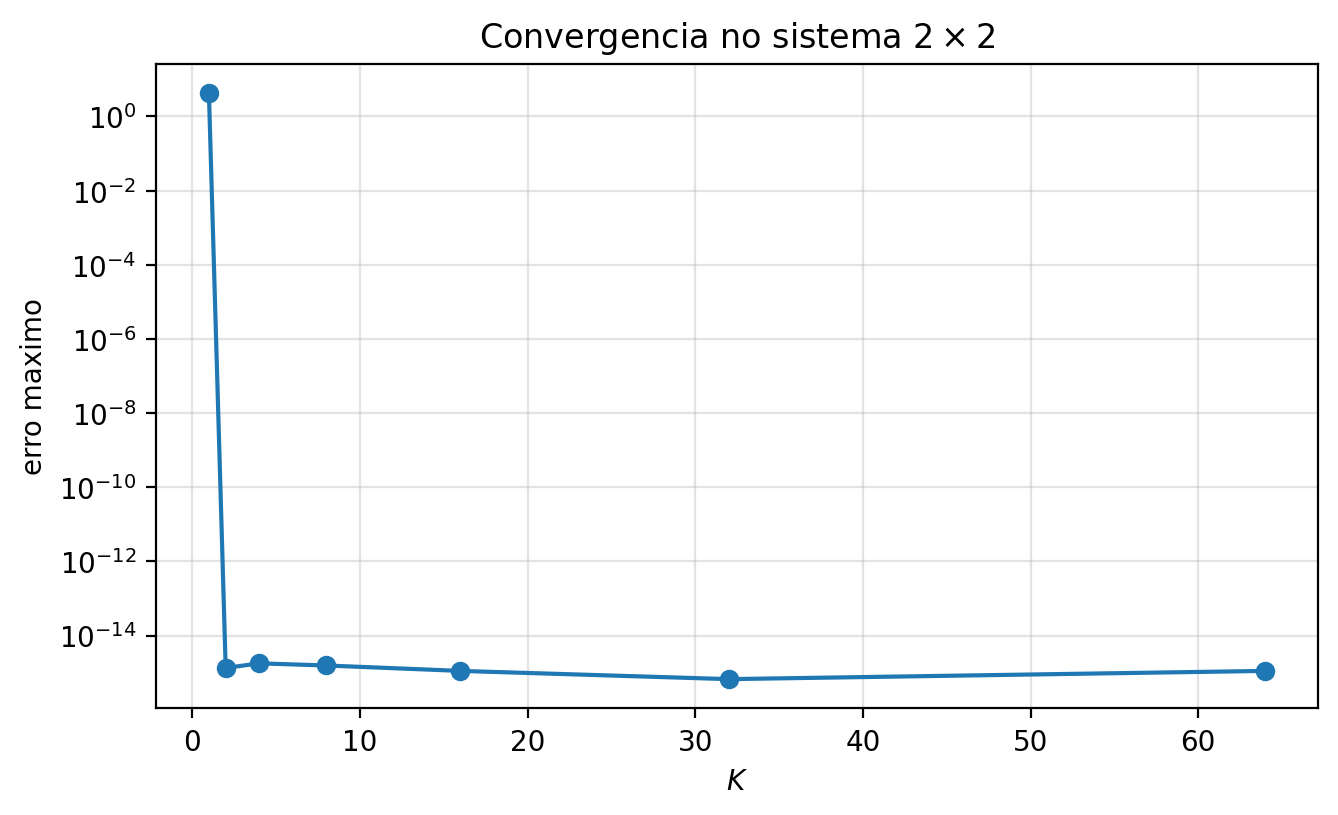
\includegraphics[width=0.78\textwidth]{figuras/grafico_convergencia_sistema2x2.png}
\caption{Convergência do erro máximo no sistema \(2\times2\) em função do número de modos de Fourier.}
\label{fig:convergencia_sistema2x2}
\end{figure}

A Figura~\ref{fig:erro_sistema2x2_k8} apresenta o erro ao longo do tempo para \(K=8\). Observa-se que o erro permanece da ordem de \(10^{-15}\), confirmando que a solução reconstruída coincide com a solução exata até erros de arredondamento.

\begin{figure}[h!]
\centering
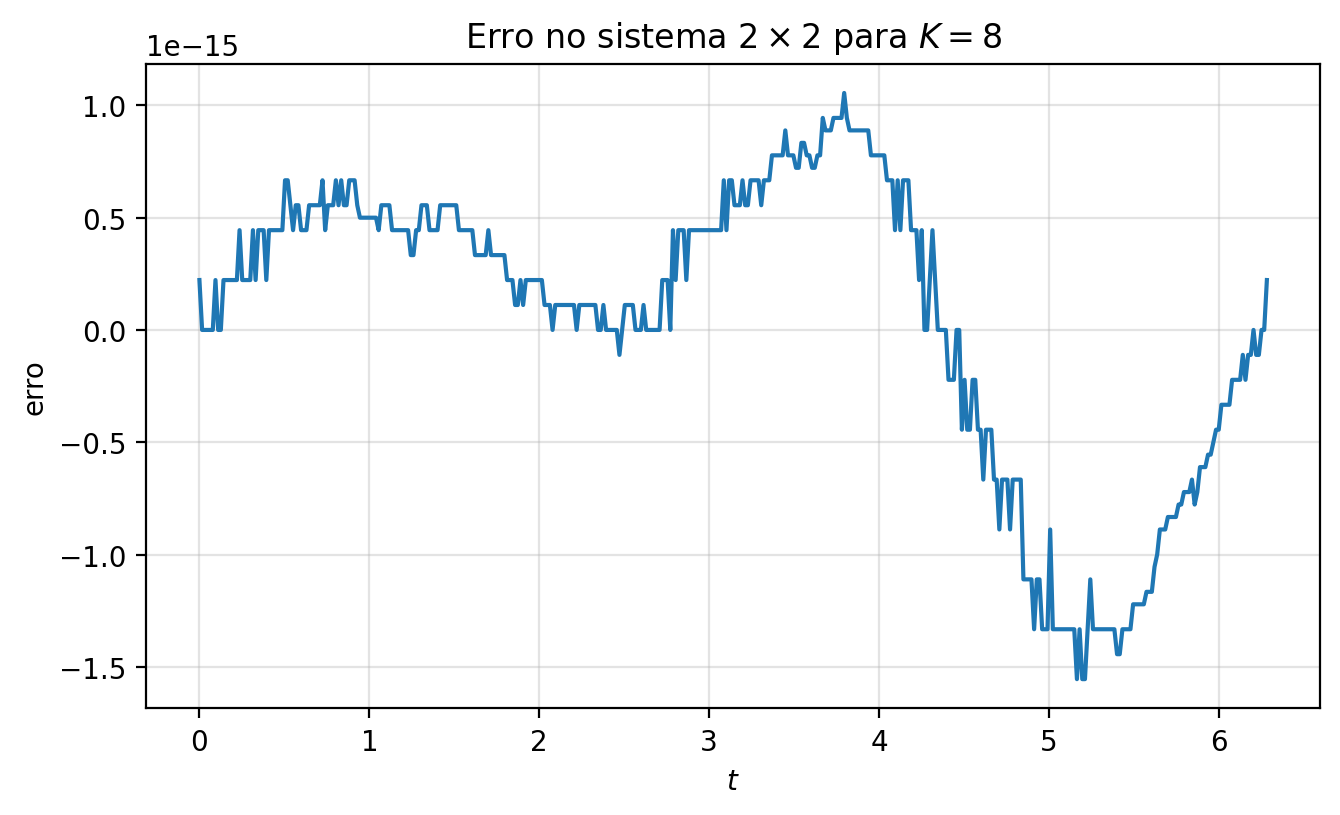
\includegraphics[width=0.78\textwidth]{figuras/grafico_erro_sistema2x2_K8.png}
\caption{Erro na primeira componente do sistema \(2\times2\) para \(K=8\).}
\label{fig:erro_sistema2x2_k8}
\end{figure}

Além do erro, calcula-se o resíduo
\[
R_K(t)=X_K'(t)-AX_K(t)-b(t),
\]
que mede o quanto a solução aproximada satisfaz o sistema diferencial. A Figura~\ref{fig:residuo_sistema2x2} mostra que, a partir de \(K=2\), o resíduo também permanece próximo da precisão de máquina. Esse resultado é importante porque, em problemas sem solução exata conhecida, o resíduo passa a ser um dos principais critérios de validação.

\begin{figure}[h!]
\centering
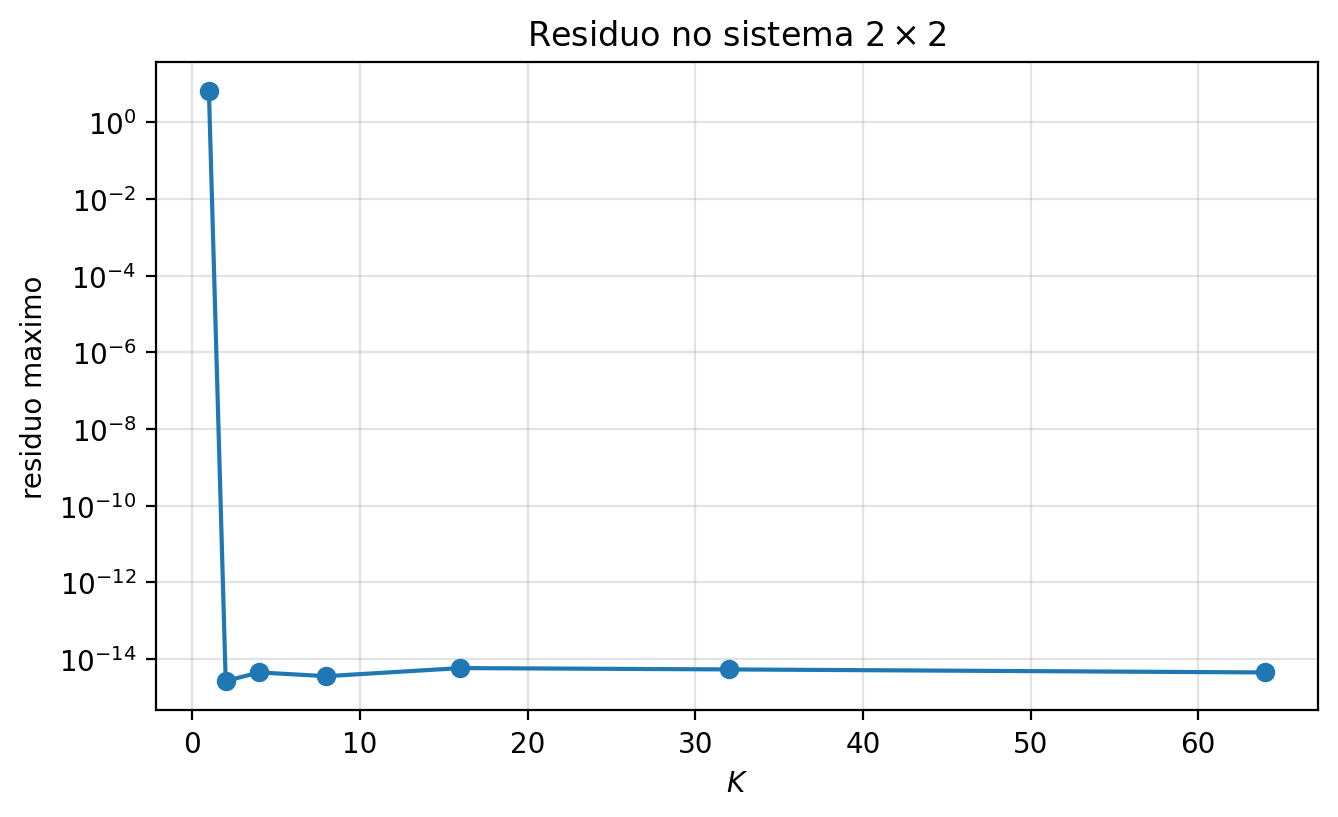
\includegraphics[width=0.78\textwidth]{figuras/grafico_residuo_sistema2x2.png}
\caption{Resíduo máximo do sistema \(2\times2\) em função de \(K\).}
\label{fig:residuo_sistema2x2}
\end{figure}

\section{Conexão entre os dois códigos}
\label{sec:conexao-codigos}

A passagem do primeiro problema de validação para o segundo problema não representa uma mudança de método, mas uma ampliação natural da mesma ideia algorítmica. No primeiro teste, parte-se diretamente de um sistema linear finito-dimensional da forma
\[
U'(t)=AU(t)+b(t),
\]
no qual a matriz \(A\) é pequena e dada explicitamente. Esse problema permite validar, de maneira isolada, a etapa temporal do método: a decomposição em modos de Fourier, o cálculo dos coeficientes da forçante por FFT, a resolução dos sistemas lineares modo a modo e a reconstrução da solução periódica.

No segundo código, o ponto de partida é a equação do calor bidimensional periódica no tempo,
\[
u_t=\Delta u+f,
\]
definida em um domínio espacial limitado. Nesse caso, antes de aplicar Fourier na variável temporal, é necessário discretizar o operador espacial \(\Delta\). Essa discretização é feita por colocação espectral de Chebyshev nas variáveis espaciais. Como consequência, a EDP é transformada em um sistema semidiscreto de equações diferenciais ordinárias no tempo,
\[
U'(t)=AU(t)+b(t),
\]
em que \(U(t)\) contém os valores aproximados da solução nos pontos internos da malha de Chebyshev, \(A\) representa o Laplaciano discreto e \(b(t)\) representa a forçante avaliada nesses mesmos pontos.

Dessa forma, depois da discretização espacial, reaparece exatamente a mesma estrutura algébrica estudada no sistema finito-dimensional. A diferença é que, no primeiro código, a matriz \(A\) é uma matriz \(2\times2\) escolhida a partir de uma equação diferencial ordinária de segunda ordem; no segundo código, \(A\) é uma matriz de dimensão maior, construída a partir das matrizes de diferenciação de Chebyshev e da soma de Kronecker que representa o Laplaciano bidimensional.

Assim, o elo central entre os dois códigos pode ser resumido por
\[
\text{EDP do calor}
\quad \xrightarrow{\text{Chebyshev no espaço}} \quad
U'(t)=AU(t)+b(t)
\quad \xrightarrow{\text{Fourier no tempo}} \quad
(ik\omega I-A)\widehat{U}_k=\widehat{b}_k.
\]
Portanto, o primeiro código valida o núcleo temporal do algoritmo, enquanto o segundo mostra como esse núcleo é incorporado a uma formulação Fourier--Chebyshev para uma equação diferencial parcial.

A Figura~\ref{fig:conexao-codigos} resume essa relação entre as duas implementações.

\begin{figure}[h!]
\centering
\begin{tikzpicture}[
    node distance=0.78cm,
    >=Latex,
    bloco/.style={
        rectangle,
        rounded corners,
        draw,
        align=center,
        minimum width=7.8cm,
        minimum height=0.82cm,
        font=\small
    },
    seta/.style={->, thick}
]

\node[bloco] (c1) {Código 1: sistema finito-dimensional\\
\(U'(t)=AU(t)+b(t)\)};

\node[bloco, below=of c1] (four1) {Validação da etapa temporal\\
Fourier no tempo, FFT para \(\widehat{b}_k\) e resolução de\\
\((ik\omega I-A)\widehat{U}_k=\widehat{b}_k\)};

\node[bloco, below=of four1] (edp) {Código 2: equação do calor bidimensional periódica\\
\(u_t=\Delta u+f\)};

\node[bloco, below=of edp] (cheb) {Discretização espacial por Chebyshev\\
colocação espectral nos pontos internos};

\node[bloco, below=of cheb] (semi) {Sistema semidiscreto resultante\\
\(U'(t)=AU(t)+b(t)\)};

\node[bloco, below=of semi] (four2) {Aplicação da mesma etapa temporal\\
Fourier no tempo, FFT e resolução modal};

\draw[seta] (c1) -- (four1);
\draw[seta] (four1) -- (edp);
\draw[seta] (edp) -- (cheb);
\draw[seta] (cheb) -- (semi);
\draw[seta] (semi) -- (four2);

\end{tikzpicture}
\caption{Conexão entre o problema finito-dimensional e a formulação Fourier--Chebyshev para a equação do calor.}
\label{fig:conexao-codigos}
\end{figure}

\section{Equação do calor bidimensional periódica}

\subsection{Formulação Fourier--Chebyshev}

Como segundo problema de teste, considera-se a equação do calor bidimensional
\[
u_t(x,y,t)=\Delta u(x,y,t)+f(x,y,t),
\qquad (x,y)\in(-1,1)\times(-1,1),
\]
com condições de contorno homogêneas de Dirichlet na fronteira e periodicidade temporal de período \(T=2\pi\):
\[
u(x,y,t+2\pi)=u(x,y,t).
\]
Esse problema representa a etapa em que a formulação temporal de Fourier, previamente validada em um sistema finito-dimensional, passa a ser combinada com uma discretização espectral espacial. A escolha de uma solução fabricada suave é deliberada: nesse regime, os coeficientes espectrais tendem a decair rapidamente, favorecendo o comportamento de convergência espectral descrito na Seção~\ref{sec:decaimento-aliasing-gibbs}.

Para discretizar o espaço, utilizam-se pontos de Chebyshev--Gauss--Lobatto. Se \(N_M\) é o parâmetro de discretização espacial, consideram-se os pontos
\[
x_j=\cos\left(\frac{j\pi}{N_M}\right),
\qquad j=0,1,\dots,N_M.
\]
Como a condição de contorno é homogênea de Dirichlet, os valores da solução na fronteira já são conhecidos e iguais a zero. Portanto, as incógnitas numéricas são tomadas apenas nos pontos internos.

A matriz de diferenciação de Chebyshev \(D\) aproxima a derivada primeira nos pontos de colocação, e \(D^2\) aproxima a derivada segunda. Após remover as linhas e colunas associadas aos pontos de fronteira, constrói-se o Laplaciano discreto bidimensional por soma de Kronecker:
\[
A=I\otimes D^2+D^2\otimes I.
\]
Assim, a equação do calor é transformada no sistema semidiscreto
\[
U'(t)=AU(t)+b(t),
\]
em que \(U(t)\) contém os valores aproximados de \(u(x_i,y_j,t)\) nos pontos internos, e \(b(t)\) contém os valores da forçante nesses mesmos pontos.

Como o problema é periódico no tempo, introduz-se
\[
\omega=\frac{2\pi}{T}
\]
e procuram-se aproximações truncadas da forma
\[
U_K(t)=\sum_{k=-K}^{K}\widehat{U}_k e^{ik\omega t},
\qquad
b_K(t)=\sum_{k=-K}^{K}\widehat{b}_k e^{ik\omega t}.
\]
Substituindo no sistema semidiscreto, obtém-se, para cada modo temporal,
\[
(ik\omega I-A)\widehat{U}_k=\widehat{b}_k,
\qquad k=-K,\dots,K.
\]
Portanto, a EDP periódica é reduzida a uma família finita de sistemas lineares independentes, um para cada frequência temporal considerada.

\subsection{Validação por solução fabricada}

Para validar o método, escolhe-se a solução exata
\[
u_{\mathrm{ex}}(x,y,t)
=
-\cos(t)\sin\bigl(\pi\cos(\pi x)\bigr)
\sin\bigl(\pi\cos(\pi y)\bigr).
\]
Essa função é \(2\pi\)-periódica no tempo, pois depende de \(\cos(t)\). Além disso, satisfaz as condições homogêneas de Dirichlet na fronteira. De fato, se \(x=\pm1\), então
\[
\cos(\pi x)=\cos(\pm\pi)=-1
\]
e, portanto,
\[
\sin(\pi\cos(\pi x))=\sin(-\pi)=0.
\]
Logo, \(u_{\mathrm{ex}}(\pm1,y,t)=0\). O mesmo raciocínio vale para \(y=\pm1\).

A forçante é obtida por substituição direta na equação do calor:
\[
f=u_t-\Delta u.
\]
Escrevendo
\[
g(x)=\sin\bigl(\pi\cos(\pi x)\bigr),
\qquad
h(y)=\sin\bigl(\pi\cos(\pi y)\bigr),
\]
temos
\[
u_{\mathrm{ex}}(x,y,t)=-\cos(t)g(x)h(y),
\]
logo
\[
u_t(x,y,t)=\sin(t)g(x)h(y).
\]
As derivadas espaciais \(u_{xx}\) e \(u_{yy}\) são calculadas analiticamente e implementadas na rotina da forçante. Esse procedimento, conhecido como solução fabricada, permite validar o método em um caso no qual a solução exata é conhecida previamente.

\subsection{Resultados obtidos}

Nos experimentos desta etapa, manteve-se fixo \(K=8\) para a aproximação de Fourier no tempo e variou-se o número de pontos de Chebyshev na discretização espacial. Essa escolha permite observar de maneira mais direta o efeito do refinamento espacial na precisão do método, uma vez que a dependência temporal da solução exata envolve essencialmente o fator \(-\cos(t)\).

Os resultados obtidos estão resumidos na Tabela~\ref{tab:calor2d}. Nesta versão, o erro principal é o erro máximo absoluto
\[
erro_{\max}=\max |U_{\mathrm{aprox}}-U_{\mathrm{ex}}|,
\]
calculado sobre todos os pontos internos e todos os tempos da malha de Fourier. Essa métrica é mais direta para avaliar a maior discrepância ponto a ponto entre a solução aproximada e a solução fabricada. A soma total dos erros em norma \(1\), usada em versões preliminares do experimento, foi mantida apenas como diagnóstico secundário, pois cresce com o número de pontos da malha e não mede diretamente o maior erro pontual.

\begin{table}[h!]
\centering
\caption{Desempenho numérico da formulação Fourier--Chebyshev para a equação do calor bidimensional periódica, com \(K=8\).}
\label{tab:calor2d}
\begin{tabular}{cccc}
\toprule
\(N_{\text{Cheb}}\) & Condição máxima & Erro máximo absoluto & Erro \(L^1\) total \\
\midrule
8  & \(1.8242\times 10^{2}\) & \(2.7111\times 10^{0}\)  & \(3.8747\times 10^{2}\) \\
16 & \(2.6766\times 10^{3}\) & \(2.0527\times 10^{-2}\) & \(8.4757\times 10^{0}\) \\
32 & \(4.1914\times 10^{4}\) & \(1.1682\times 10^{-6}\) & \(2.0972\times 10^{-3}\) \\
60 & \(5.0538\times 10^{5}\) & \(1.75\times 10^{-14}\) & \(\mathcal{O}(10^{-10})\) \\
80 & \(1.60\times 10^{6}\)  & \(2.53\times 10^{-14}\) & \(\mathcal{O}(10^{-10})\) \\
\bottomrule
\end{tabular}
\end{table}

A distinção entre as duas últimas colunas é importante. Os valores anteriormente reportados como erro principal correspondiam, na prática, ao diagnóstico acumulado em norma \(1\). Após a correção, o erro máximo absoluto mostra diretamente a maior diferença ponto a ponto entre a solução numérica e a solução fabricada. Esse ajuste torna a interpretação dos resultados mais clara e compatível com a métrica usual de erro em norma infinito.

Os resíduos máximos permaneceram próximos da precisão de máquina, com valores da ordem de \(10^{-13}\) a \(10^{-11}\), indicando que os sistemas lineares modais foram resolvidos de modo consistente. Para os maiores valores de \(N_{\text{Cheb}}\), as pequenas variações numéricas são dominadas por arredondamento e pelo aumento do condicionamento.

A Figura~\ref{fig:erro_calor2d_ncheb} mostra a queda do erro máximo com o refinamento espacial. Observa-se que o erro passa de valores da ordem de \(10^0\), para \(N_{\text{Cheb}}=8\), para valores próximos da precisão de máquina quando \(N_{\text{Cheb}}\) é aumentado. Essa redução acentuada é compatível com o comportamento esperado de métodos espectrais quando aplicados a soluções suficientemente regulares. A pequena perda relativa de estabilidade observada no regime de erro de máquina é coerente com o crescimento do condicionamento das matrizes espectrais.

\begin{figure}[h!]
\centering
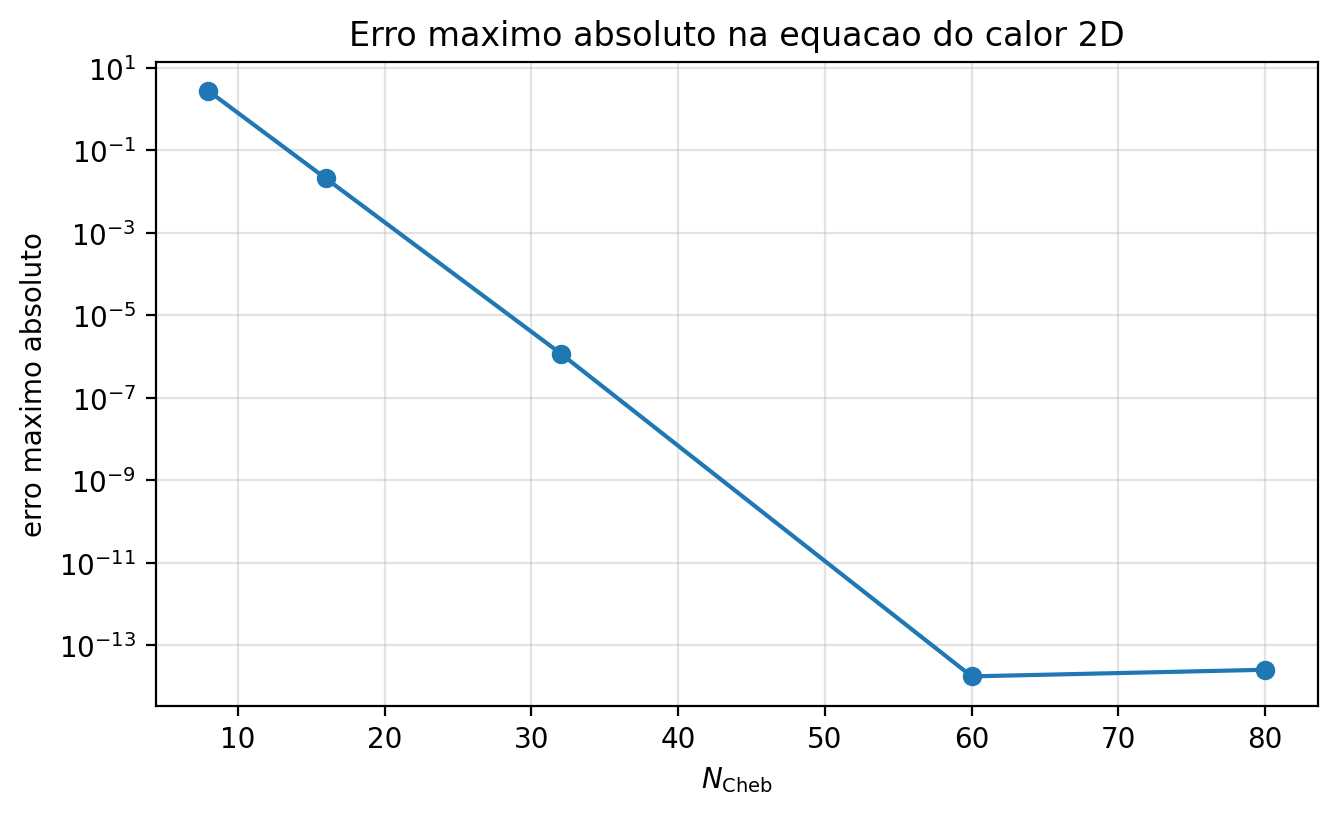
\includegraphics[width=0.78\textwidth]{figuras/grafico_erro_calor2d.png}
\caption{Erro máximo absoluto em função do número de pontos de Chebyshev para a equação do calor bidimensional.}
\label{fig:erro_calor2d_ncheb}
\end{figure}

A principal razão para essa queda rápida está na suavidade da solução exata e na adequação dos pontos de Chebyshev para representar funções regulares em intervalos limitados. Como a solução fabricada contém fatores espaciais suaves da forma
\[
\sin\bigl(\pi\cos(\pi x)\bigr)
\quad \text{e} \quad
\sin\bigl(\pi\cos(\pi y)\bigr),
\]
o aumento de \(N_{\text{Cheb}}\) permite capturar com maior precisão a estrutura espacial da solução.

Por outro lado, a Figura~\ref{fig:cond_calor2d_ncheb} mostra que o número de condição dos sistemas modais cresce significativamente com o refinamento espacial. Esse comportamento é típico de métodos espectrais baseados em matrizes de diferenciação, pois as matrizes associadas a operadores diferenciais tornam-se progressivamente mais mal condicionadas à medida que o número de pontos aumenta.

\begin{figure}[h!]
\centering
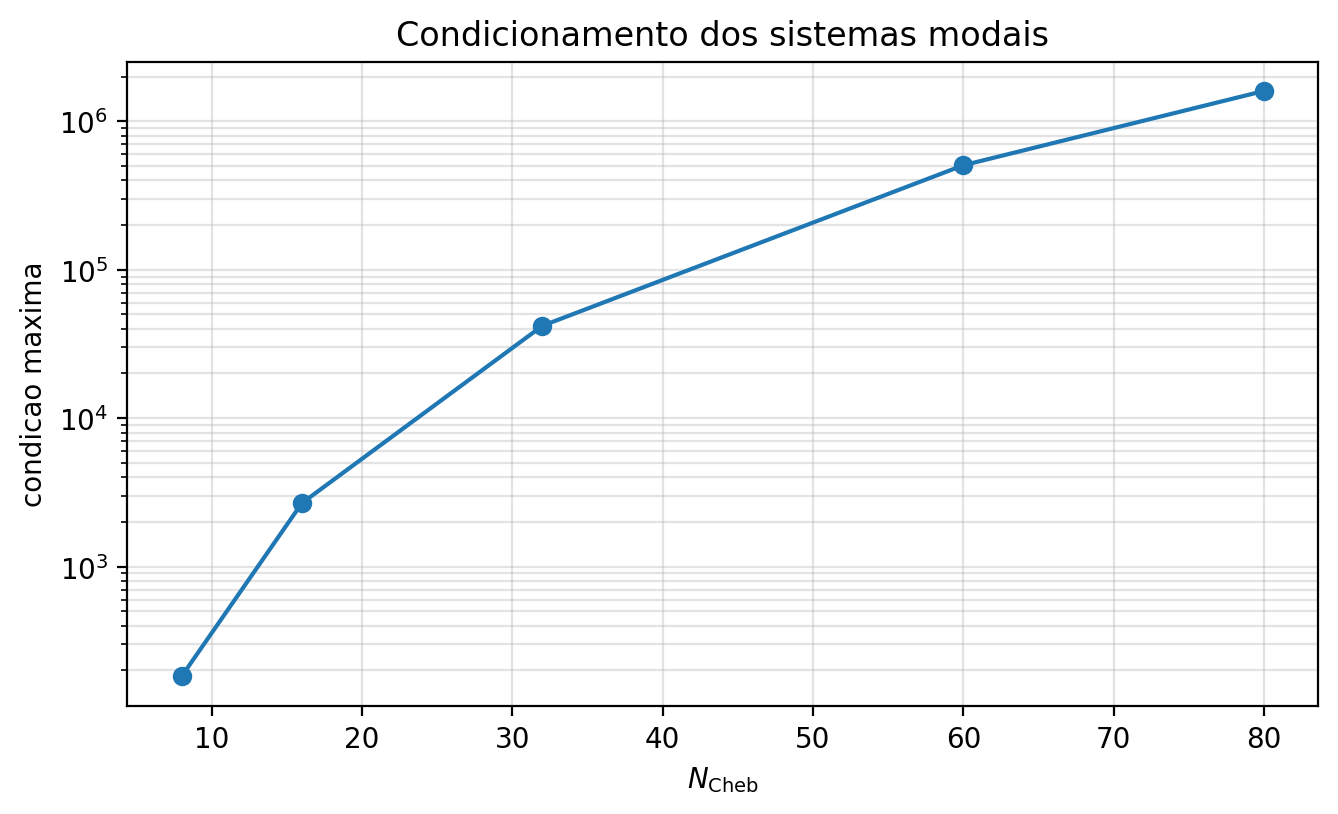
\includegraphics[width=0.78\textwidth]{figuras/grafico_condicao_calor2d.png}
\caption{Número de condição máximo dos sistemas modais em função de \(N_{\text{Cheb}}\).}
\label{fig:cond_calor2d_ncheb}
\end{figure}

A análise conjunta do erro e do condicionamento é apresentada na Figura~\ref{fig:erro_cond_calor2d}. Observa-se um compromisso entre precisão e estabilidade numérica: o aumento de \(N_{\text{Cheb}}\) melhora a representação espacial da solução, mas também torna os sistemas lineares mais sensíveis a erros de arredondamento.

\begin{figure}[h!]
\centering
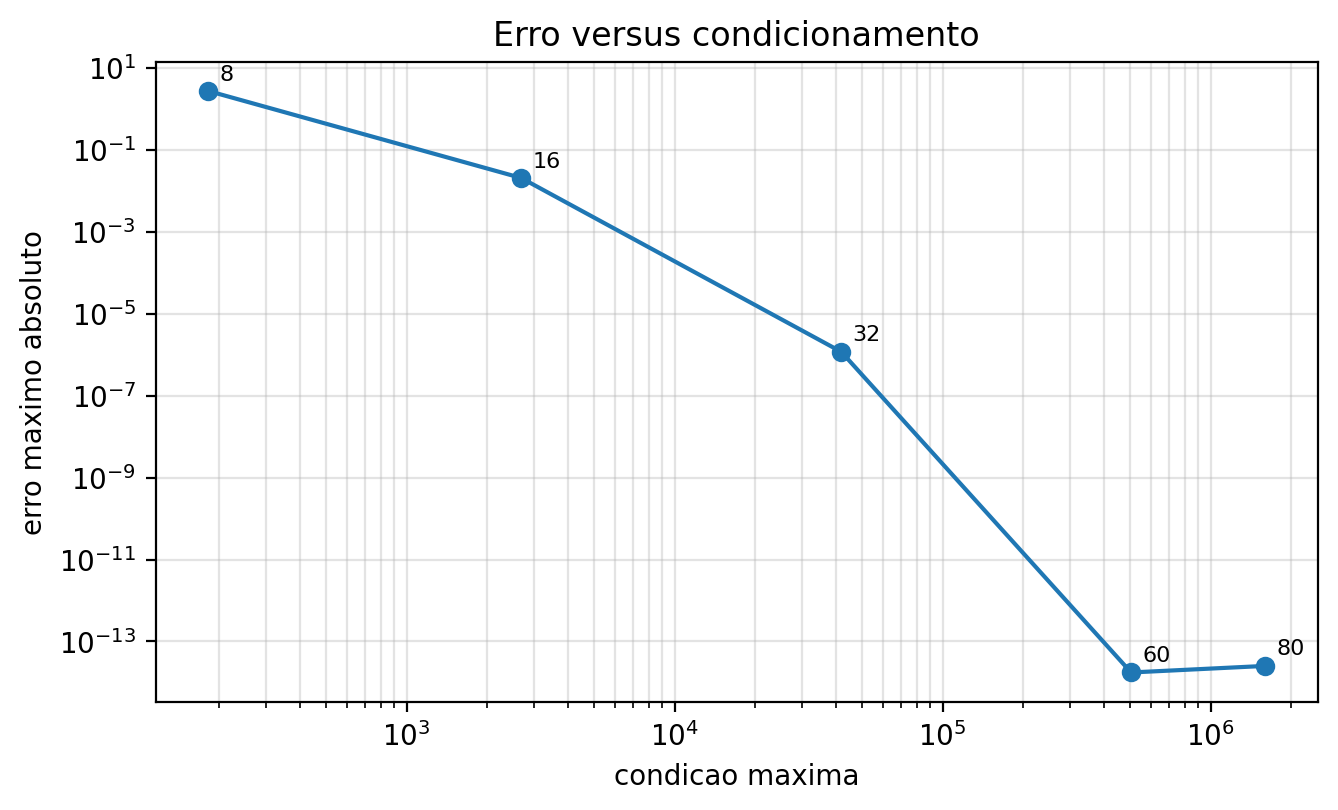
\includegraphics[width=0.78\textwidth]{figuras/grafico_erro_vs_condicao_calor2d.png}
\caption{Relação entre erro máximo absoluto e número de condição máximo na formulação Fourier--Chebyshev.}
\label{fig:erro_cond_calor2d}
\end{figure}

Apesar do crescimento do condicionamento, os resíduos permanecem próximos da precisão de máquina, como mostra a Figura~\ref{fig:residuo_calor2d}. Isso indica que os sistemas lineares modais foram resolvidos de maneira consistente e que a solução reconstruída satisfaz o sistema semidiscreto com alta acurácia.

\begin{figure}[h!]
\centering
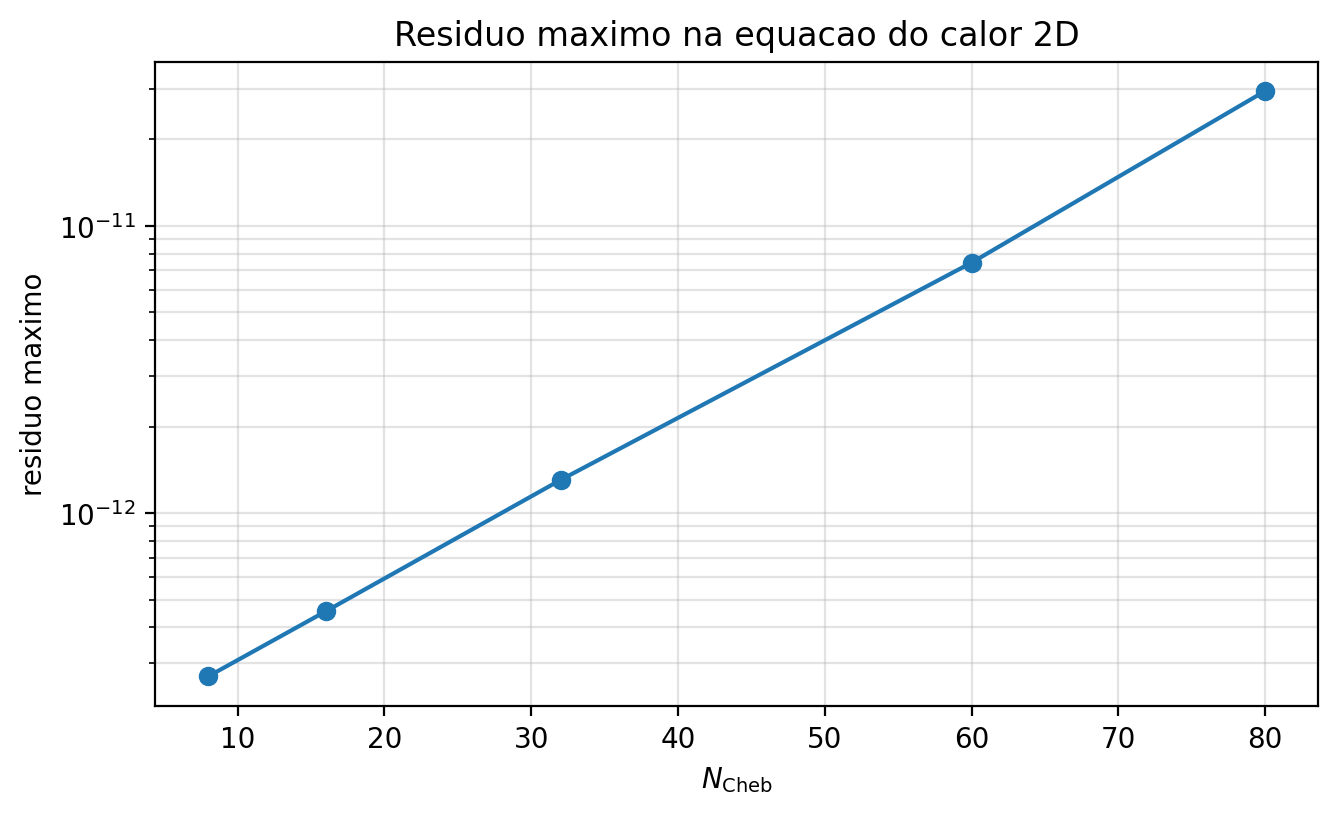
\includegraphics[width=0.78\textwidth]{figuras/grafico_residuo_calor2d.png}
\caption{Resíduo máximo da equação do calor bidimensional em função de \(N_{\text{Cheb}}\).}
\label{fig:residuo_calor2d}
\end{figure}

As superfícies da solução aproximada e do erro espacial fornecem uma visualização qualitativa do refinamento. As Figuras~\ref{fig:solucao_calor_n8}, \ref{fig:solucao_calor_n16} e \ref{fig:solucao_calor_n32} mostram a solução aproximada no instante \(t=0\) para diferentes valores de \(N_{\text{Cheb}}\). Com o aumento da resolução espacial, a superfície passa a representar melhor a estrutura oscilatória da solução fabricada.

\begin{figure}[h!]
\centering
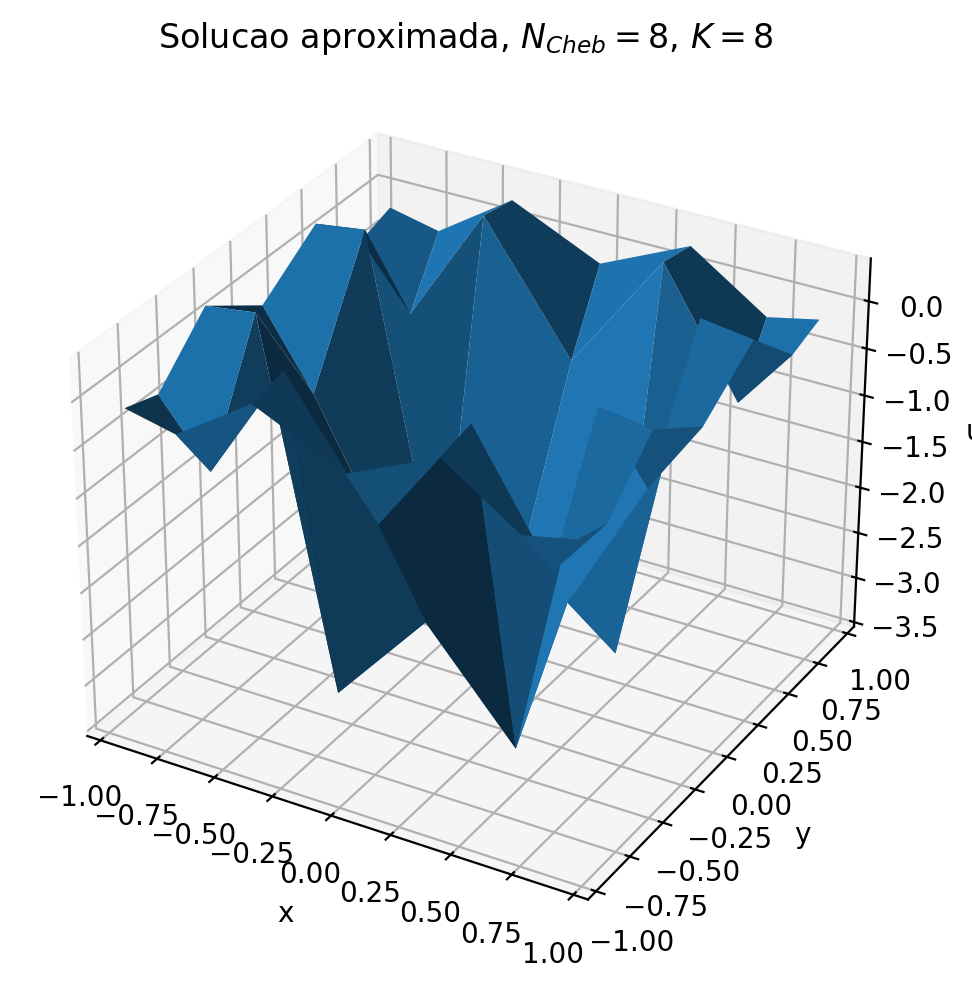
\includegraphics[width=0.72\textwidth]{figuras/superficie_solucao_calor2d_N8_K8.png}
\caption{Solução aproximada no instante \(t=0\), com \(N_{\text{Cheb}}=8\) e \(K=8\).}
\label{fig:solucao_calor_n8}
\end{figure}

\begin{figure}[h!]
\centering
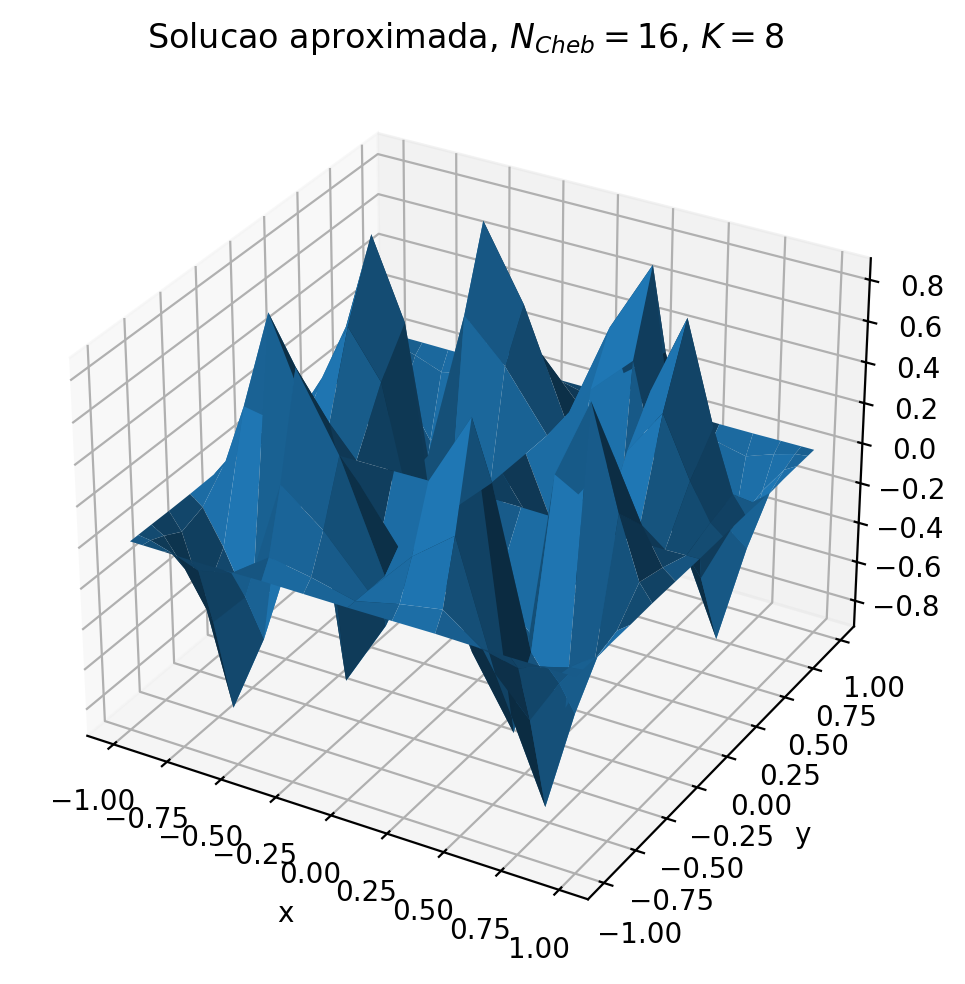
\includegraphics[width=0.72\textwidth]{figuras/superficie_solucao_calor2d_N16_K8.png}
\caption{Solução aproximada no instante \(t=0\), com \(N_{\text{Cheb}}=16\) e \(K=8\).}
\label{fig:solucao_calor_n16}
\end{figure}

\begin{figure}[h!]
\centering
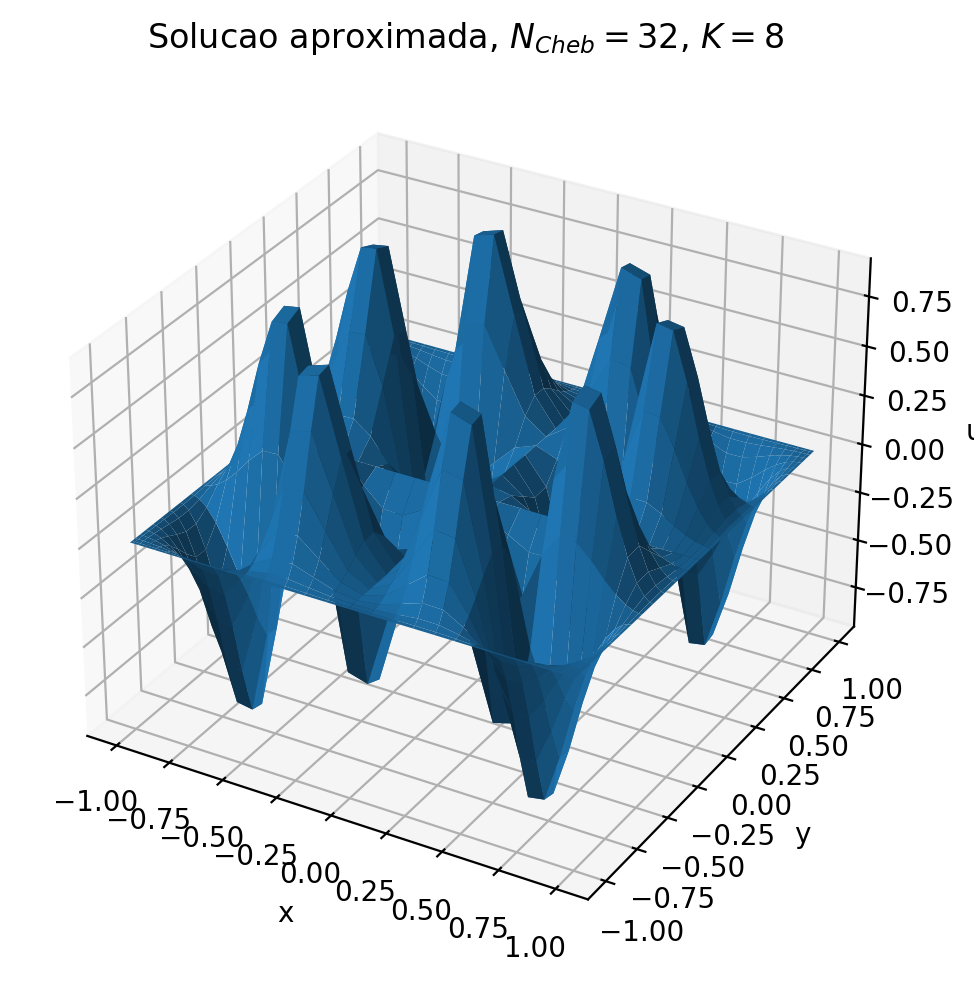
\includegraphics[width=0.72\textwidth]{figuras/superficie_solucao_calor2d_N32_K8.png}
\caption{Solução aproximada no instante \(t=0\), com \(N_{\text{Cheb}}=32\) e \(K=8\).}
\label{fig:solucao_calor_n32}
\end{figure}

As Figuras~\ref{fig:erro_espacial_n8}, \ref{fig:erro_espacial_n16} e \ref{fig:erro_espacial_n32} mostram o erro espacial correspondente. Para \(N_{\text{Cheb}}=8\), o erro ainda é elevado. Para \(N_{\text{Cheb}}=16\), observa-se redução significativa. Para \(N_{\text{Cheb}}=32\), o erro atinge valores muito pequenos, da ordem de \(10^{-6}\) na malha considerada, confirmando a melhora da aproximação com o refinamento espacial.

\begin{figure}[h!]
\centering
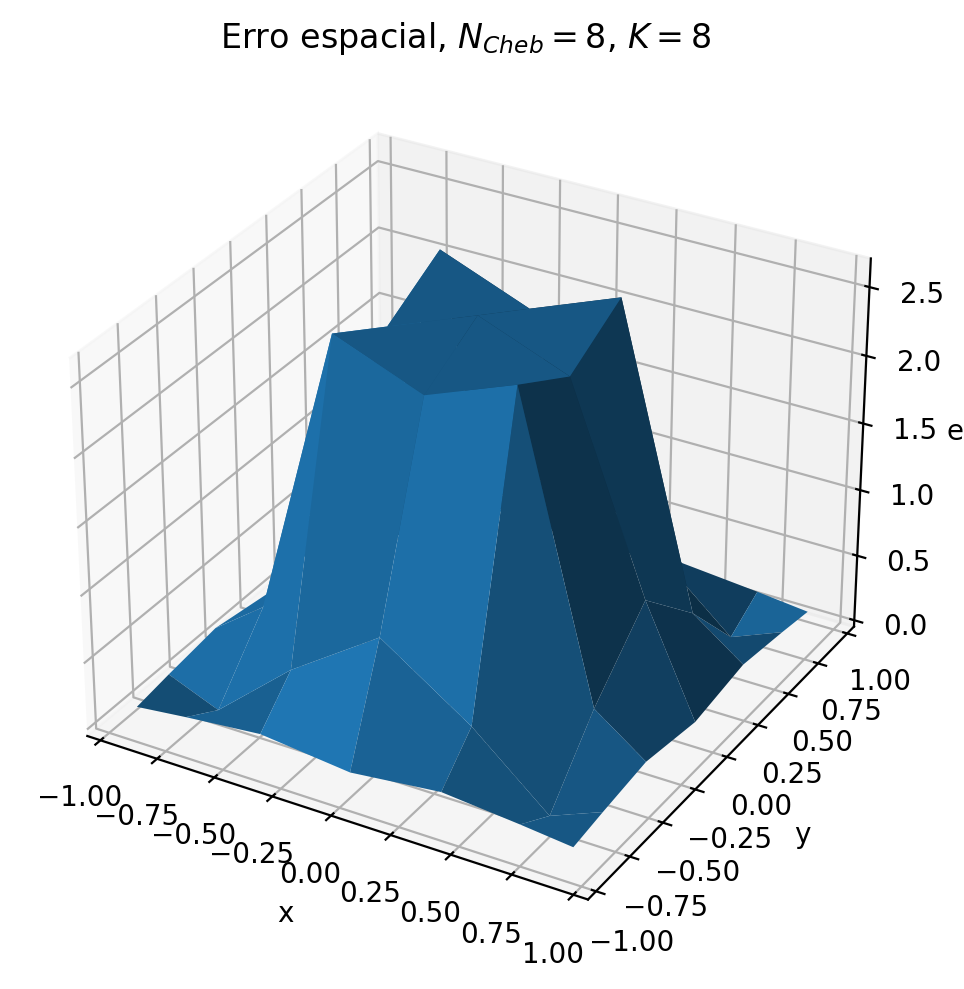
\includegraphics[width=0.72\textwidth]{figuras/superficie_erro_calor2d_N8_K8.png}
\caption{Erro espacial no instante \(t=0\), com \(N_{\text{Cheb}}=8\) e \(K=8\).}
\label{fig:erro_espacial_n8}
\end{figure}

\begin{figure}[h!]
\centering
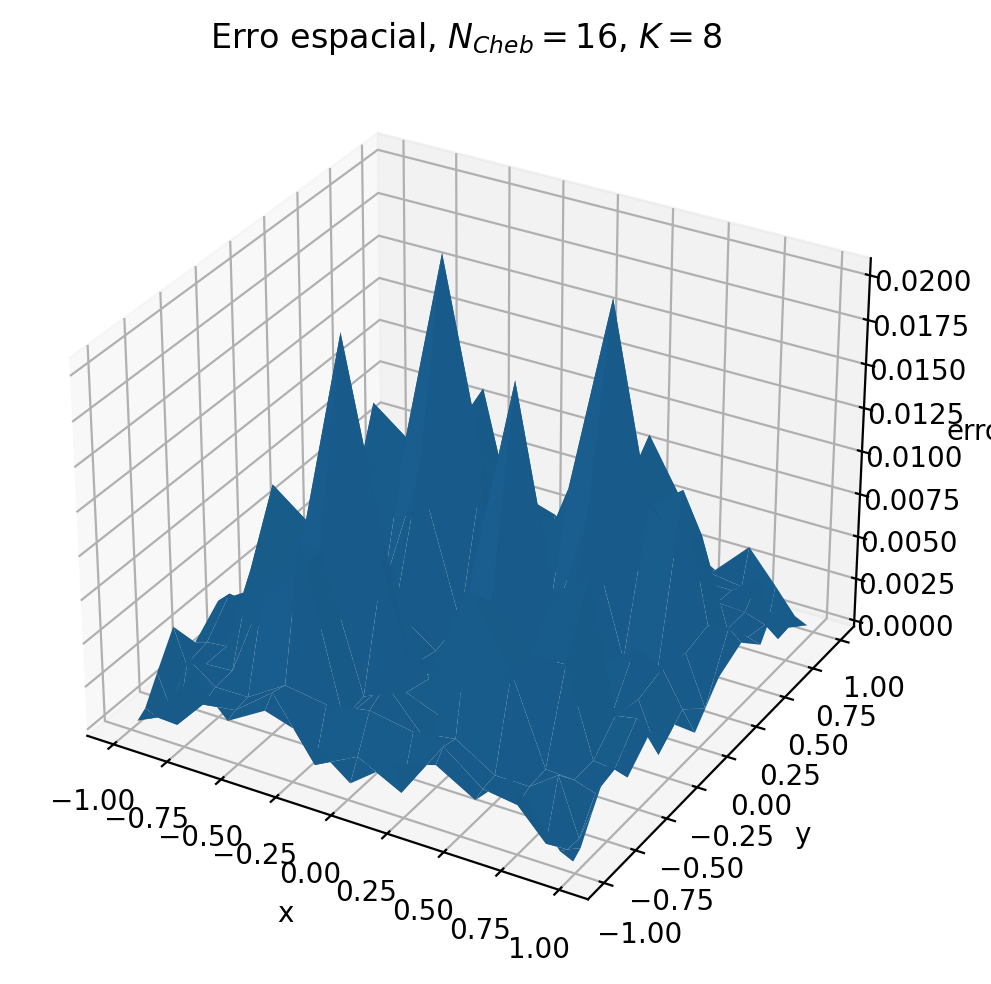
\includegraphics[width=0.72\textwidth]{figuras/superficie_erro_calor2d_N16_K8.png}
\caption{Erro espacial no instante \(t=0\), com \(N_{\text{Cheb}}=16\) e \(K=8\).}
\label{fig:erro_espacial_n16}
\end{figure}

\begin{figure}[h!]
\centering
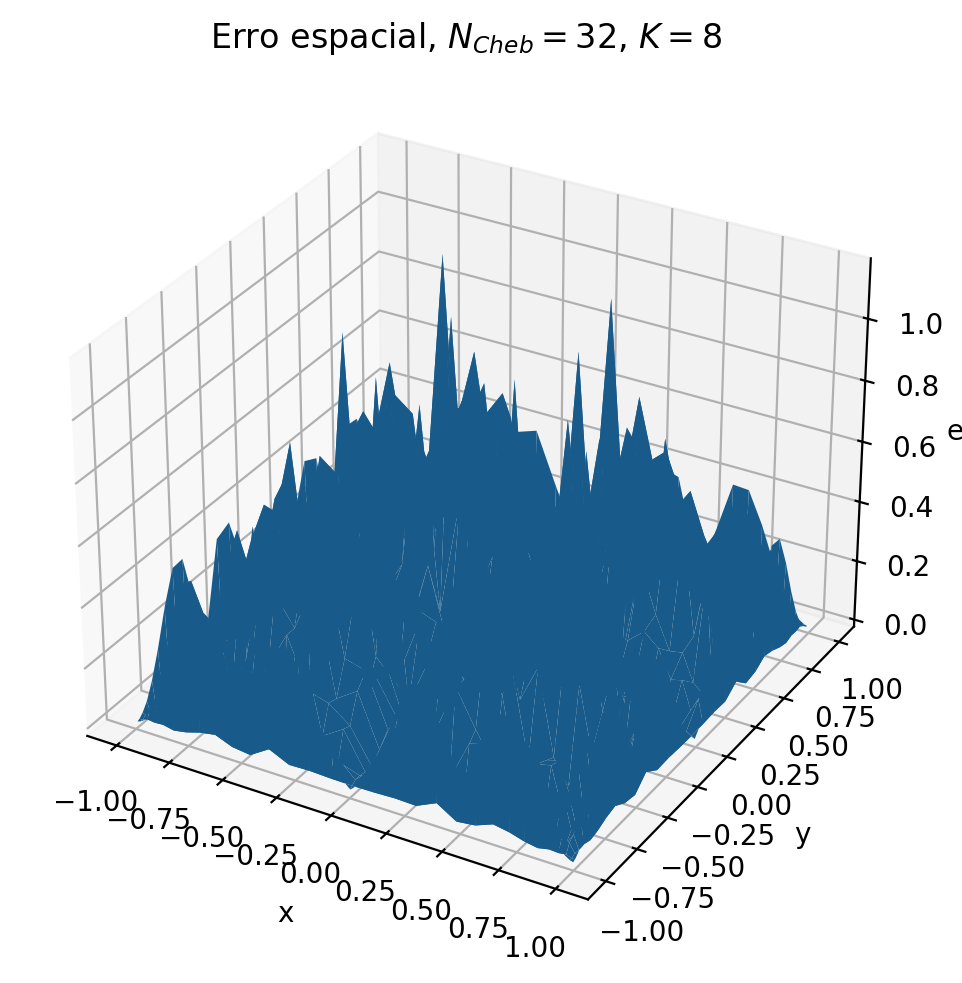
\includegraphics[width=0.72\textwidth]{figuras/superficie_erro_calor2d_N32_K8.png}
\caption{Erro espacial no instante \(t=0\), com \(N_{\text{Cheb}}=32\) e \(K=8\).}
\label{fig:erro_espacial_n32}
\end{figure}

\section{Síntese dos resultados}

Os experimentos numéricos confirmam a coerência da formulação proposta. O teste \(2\times2\) valida a etapa temporal baseada em Fourier, mostrando que poucos modos são suficientes quando a solução possui estrutura harmônica simples. Nesse caso, a solução exata contém apenas os harmônicos \(k=1\) e \(k=2\); por isso, a partir de \(K=2\), a aproximação passa a conter todos os modos relevantes e o erro cai para a ordem da precisão de máquina.

O problema da equação do calor bidimensional evidencia a eficácia da combinação Fourier--Chebyshev. Como a solução fabricada é suave no espaço e periódica no tempo, observa-se o comportamento esperado para métodos espectrais: o erro máximo absoluto decresce rapidamente com o refinamento espacial. Essa queda acentuada está associada ao rápido decaimento dos coeficientes espectrais de funções regulares e à adequação dos pontos de Chebyshev--Gauss--Lobatto para domínios limitados.

Ao mesmo tempo, os resultados mostram uma limitação importante: o ganho de precisão obtido com o aumento de \(N_{\text{Cheb}}\) vem acompanhado do crescimento do número de condição dos sistemas lineares. Esse comportamento é típico de formulações espectrais por colocação, especialmente quando se utilizam matrizes de diferenciação de alta ordem. Assim, os experimentos indicam não apenas a precisão da abordagem espectral, mas também a necessidade de monitorar o condicionamento e os efeitos de arredondamento em discretizações mais refinadas.

Do ponto de vista metodológico, as tabelas fornecem os valores quantitativos principais, enquanto os gráficos ajudam a interpretar a tendência dos experimentos: convergência rápida para soluções suaves, resíduos próximos da precisão de máquina e aumento do condicionamento com o refinamento. Em trabalhos futuros, uma etapa adicional natural será aplicar o mesmo procedimento a forçantes sem solução exata conhecida, usando o resíduo como principal critério de validação, e a problemas não lineares periódicos, nos quais o controle de aliasing por técnicas de \emph{dealiasing} se torna relevante.

\appendix

\chapter{Códigos comentados utilizados nas simulações}

Este apêndice reúne as versões comentadas dos códigos utilizados para gerar os resultados numéricos. O objetivo não é substituir a formulação matemática apresentada nos capítulos anteriores, mas registrar a implementação de modo transparente. Os comentários foram escritos para evidenciar a correspondência entre cada etapa computacional e a fundamentação desenvolvida no relatório: expansão de Fourier no tempo, cálculo dos coeficientes por FFT, resolução dos sistemas modais, discretização de Chebyshev no espaço, cálculo do erro e avaliação do resíduo.

\section{Código para o sistema linear periódico \texorpdfstring{\(2\times2\)}{2x2}}

O Código~\ref{lst:sistema2x2} implementa o problema de validação finito-dimensional. Nesse caso, a matriz \(A\) já é dada e o algoritmo atua diretamente sobre o sistema
\[
U'(t)=AU(t)+b(t).
\]
A finalidade desse código é testar isoladamente a etapa temporal baseada em Fourier antes de aplicá-la ao sistema semidiscreto proveniente da equação do calor.

\lstinputlisting[style=codigoIC,language=Matlab,caption={Código comentado para o sistema linear periódico \(2\times2\).},label={lst:sistema2x2}]{codigos/teste_sistema2x2_fourier_COMENTADO_ASCII.m}

\section{Código Fourier--Chebyshev para a equação do calor bidimensional}

O Código~\ref{lst:calor2d} implementa a formulação Fourier--Chebyshev para a equação do calor bidimensional periódica no tempo. A diferença fundamental em relação ao código anterior é que, neste caso, a matriz \(A\) não é escolhida livremente: ela é construída pela discretização espectral do Laplaciano espacial usando matrizes de diferenciação de Chebyshev e produtos de Kronecker. Após essa etapa, reaparece a mesma estrutura
\[
U'(t)=AU(t)+b(t),
\]
e aplica-se novamente o procedimento em modos de Fourier.

\lstinputlisting[style=codigoIC,language=Matlab,caption={Código comentado para a equação do calor 2D com Chebyshev no espaço e Fourier no tempo.},label={lst:calor2d}]{codigos/EqCalor2D_timeperiodic_SPECTRAL_COMENTADO.m}

\section{Rotina genérica para sistemas lineares periódicos}

O Código~\ref{lst:rotina-generica} apresenta uma versão genérica da rotina temporal por Fourier. Diferentemente do código de validação \(2\times2\), no qual a matriz \(A\) é fixada por um exemplo específico, esta rotina recebe a matriz \(A\) e a função vetorial periódica \(b(t)\) como entradas. A função fornecida pelo usuário deve ser compatível com a dimensão de \(A\), isto é, se \(A\in\mathbb{R}^{n\times n}\), então \(b(t)\in\mathbb{R}^n\). Além disso, espera-se que \(b(t)\) seja \(T\)-periódica e suficientemente regular para que a aproximação por Fourier seja eficiente.

A rotina também calcula o resíduo
\[
R_K(t)=U_K'(t)-AU_K(t)-b(t),
\]
bem como o maior número de condição dos sistemas modais. Esses diagnósticos são importantes para verificar se a solução aproximada satisfaz a equação diferencial e se os sistemas lineares associados aos modos de Fourier estão bem condicionados.

\lstinputlisting[style=codigoIC,language=Matlab,caption={Rotina genérica comentada para sistemas lineares periódicos.},label={lst:rotina-generica}]{codigos/periodic_solution_fourier_generico.m}

\section{Exemplo de uso da rotina genérica}

O Código~\ref{lst:exemplo-generico} mostra como utilizar a rotina genérica no caso do sistema \(2\times2\). Nesse exemplo, o usuário fornece a matriz \(A\), a função periódica \(b(t)\) e uma solução exata para validação. Essa estrutura permite reaproveitar a mesma rotina para outros sistemas lineares periódicos, alterando apenas os dados de entrada.

\lstinputlisting[style=codigoIC,language=Matlab,caption={Exemplo de uso da rotina genérica no sistema \(2\times2\).},label={lst:exemplo-generico}]{codigos/exemplo_uso_periodic_solution_fourier_generico.m}


\section{Experimento complementar sobre regularidade em Fourier}

O Código~\ref{lst:regularidade-fourier} apresenta um experimento complementar utilizado para ilustrar a relação entre regularidade da função e convergência espectral. A função suave \(u(t)=e^{\cos t}\) é comparada com a função menos regular \(u(t)=|\sin t|\), evidenciando que funções mais suaves tendem a apresentar decaimento mais rápido dos coeficientes e, consequentemente, melhor comportamento espectral.

\lstinputlisting[style=codigoIC,language=Matlab,caption={Experimento complementar sobre regularidade e convergência de Fourier.},label={lst:regularidade-fourier}]{codigos/experimentos_regularidade_fourier_COMENTADO_ASCII.m}

\section{Script para geração das figuras}

O Código~\ref{lst:gerar-figuras} reúne os comandos utilizados para gerar as figuras chamadas no Capítulo 5. Ele salva os arquivos gráficos na pasta \texttt{figuras/}, mantendo os nomes usados nos comandos \texttt{\textbackslash includegraphics}. Esse script também registra a distinção entre o erro máximo absoluto e o diagnóstico acumulado em norma \(L^1\).

\lstinputlisting[style=codigoIC,language=Matlab,caption={Script para geração das figuras do relatório.},label={lst:gerar-figuras}]{codigos/gerar_figuras_IC.m}


\end{document}
